\documentclass[11pt,a4paper]{article}

\usepackage[T1]{fontenc}
\usepackage[utf8]{inputenc}
\usepackage[french]{babel}
\usepackage{lmodern}
\usepackage{microtype}
\usepackage{amsmath,amssymb,mathtools,amsthm}
\usepackage[a4paper,margin=2.6cm]{geometry}
\usepackage{enumitem}
\usepackage{mathrsfs}
\usepackage{booktabs}
\usepackage{array}
\usepackage{tikz}
\usetikzlibrary{arrows.meta,positioning}
\usepackage{graphicx}
\usepackage{float}
\graphicspath{{fig/}}
\usepackage{hyperref}
\hypersetup{pdftitle={IWS Volume II -- Classe, objets et transformations -- V5.17},
  pdfauthor={Benoit Hurpeau},colorlinks=true,linkcolor=black,citecolor=black,urlcolor=black}

\theoremstyle{definition}
\newtheorem{definition}{Définition}[section]
\newtheorem{candidate}[definition]{Candidat}
\newtheorem{proposition}[definition]{Proposition candidate}
\newtheorem{propositionthm}[definition]{Proposition}
\newtheorem{lemma}[definition]{Lemme}
\newtheorem{corollary}[definition]{Corollaire}
\newtheorem{question}[definition]{Question ouverte}
\theoremstyle{remark}
\newtheorem{remark}[definition]{Remarque}
\newtheorem{crashtest}[definition]{Crash-test}

\newcommand{\IWS}{\mathfrak{IWS}}
\newcommand{\Hyb}{\mathfrak H}
\newcommand{\X}{\mathcal X}
\newcommand{\Sstruct}{\mathcal S}
\newcommand{\M}{\mathfrak M}
\newcommand{\Madm}{\mathfrak M^{\mathrm{adm}}}
\newcommand{\Supp}{\operatorname{Supp}}
\newcommand{\Reach}{\operatorname{Reach}}
\newcommand{\End}{\operatorname{End}}
\newcommand{\Word}{\operatorname{Word}}
\newcommand{\Rep}{\operatorname{Rep}}
\newcommand{\Exec}{\operatorname{Exec}}
\newcommand{\Id}{\operatorname{Id}}

\title{\textbf{IWS -- Volume II}\\[0.4em]\large Classe, présentations et transformations -- V5.17}
\author{Benoit Hurpeau}
\date{\today}

\begin{document}
\maketitle

\begin{abstract}
Le premier volume construit un noyau hybride particulier et montre notamment que la trace peut modifier la dynamique future et que l'ordre des Kairos peut modifier la structure atteinte. Le présent texte cherche non plus à généraliser les équations du noyau, mais à isoler une classe minimale de systèmes présentés dont l'histoire reste capable de modifier leurs restructurations futures.

La méthode est volontairement parcimonieuse : une structure mathématique n'est ajoutée que lorsqu'un obstacle précis l'exige. La version présente distingue ainsi la dynamique hybride ambiante, la lecture déclarée, les histoires admissibles, la structure lisible, l'opacité relative à la lecture et plusieurs granularités de transformation. Elle ne suppose encore ni fibré, ni connexion, ni o-minimalité, ni temps propre. Ces objets restent des directions de recherche et non des prémisses de la définition. Pour le noyau découplé, une borne semi-algébrique de croissance inclut désormais les ties déterministes ; une annulation transverse de trace fournit en outre un premier mécanisme explicite de bifurcation des partitions lorsque le présent observable varie. Une preuve conditionnelle de transmission $C^2$ à profondeur finie est désormais accompagnée d'une certification assistée par ordinateur des huit premiers Kairos du protocole \texttt{kept1}, reproduite par une seconde méthode pour les événements et les non-annulations aux rangs 2--8 ; les quotients de factorisation au rang 1 sont certifiés par la première méthode seule. Ce résultat demeure local, sous réserve de la validité des enclosures et sans relecture par un tiers.
\end{abstract}

\section{Changement de niveau : du spécimen à la classe}

Le noyau du Volume I fournit un spécimen suffisamment précis pour être simulé et analysé. Sa dimension, son graphe, ses saturations, la forme de sa trace, ses lois de dissipation et son recâblage sont cependant des choix de réalisation. Une définition de classe ne doit pas les promouvoir en propriétés constitutives sans nécessité.

La question du Volume II est donc : quelles propriétés survivent lorsque l'on oublie les détails de réalisation tout en conservant ce qui fait qu'un système est reconnu comme un IWS ? La règle de méthode sera :
\[
\boxed{\text{ne rien ajouter tant qu'un défaut précis ne l'exige pas.}}
\]

Cette règle vaut en particulier pour les structures géométriques. Une projection n'est pas appelée fibré par anticipation ; une comparaison de fibres n'est pas supposée disposer d'une connexion ; une reparamétrisation temporelle n'est pas introduite avant qu'un problème de temps intrinsèque l'exige.

\section{Socle hybride ambiant}

\begin{definition}[Système hybride de base]
On considère un système
\[
S=(\X,C,F,D,K;\Exec),
\]
où $C$ est l'ensemble de flot, $F$ le générateur continu, $D$ l'ensemble de saut, $K$ l'opérateur de saut et $\Exec$ la sémantique d'exécution lorsque celle-ci ne se déduit pas sans ambiguïté des seules données $(C,F,D,K)$.
\end{definition}

Pour tout état admissible $x\in C$, on note dès maintenant $\Madm_x\subseteq\M$ l'ensemble des histoires admissibles et exécutables depuis $x$. On peut noter $\Madm=\bigcup_{x\in C}\Madm_x\subseteq\M$ l'union ensembliste des histoires admissibles quelque part. Cette union ne porte toutefois aucune information sur l'état de départ : elle ne sera jamais utilisée seule pour typer une exécution, une continuation ou un transport d'histoires.

Pour $x\in C$ et $\mathcal H\in\Madm_x$, on note explicitement
\[
\boxed{\gamma_{x,\mathcal H}:=\Exec(x,\mathcal H)}
\]
l'exécution hybride issue de $x$ sous l'histoire $\mathcal H$, définie sur son domaine hybride $\operatorname{dom}\gamma_{x,\mathcal H}\subseteq\mathbb R_{\geq0}\times\mathbb N$. Cette notation sera utilisée dans toute la suite.

On suppose un socle de bonne position : existence et unicité des phases de flot pour les entrées admissibles, déterminisme des événements et de leur ordre lorsqu'ils sont simultanés, priorité au saut lorsqu'elle appartient à la sémantique déclarée, et absence de Zénon. Ces hypothèses seront notées provisoirement H1--H4 et définissent une classe ambiante $\Hyb$. On exige en outre l'\emph{invariance d'admissibilité} : pour toute condition initiale $x_0\in C$ et toute histoire admissible $\mathcal H\in\Madm_{x_0}$, l'exécution correspondante reste dans $C$ sur tout son domaine :
\[
\boxed{x_0\in C,\ \mathcal H\in\Madm_{x_0}
\quad\Longrightarrow\quad
\gamma_{x_0,\mathcal H}(t,j)\in C.}
\]
Cette propriété appartient au socle. Dans un modèle concret, elle peut être démontrée par des conditions suffisantes plus élémentaires : fermeture de $C$ et $D$, priorité au premier contact lorsqu'elle est déclarée, couverture de la frontière dynamique de sortie par $D$, et $K(C\cap D)\subseteq C$. Ces conditions suffisantes ne sont pas confondues avec la propriété d'invariance elle-même.

Elles ne caractérisent pas un IWS. Elles rendent seulement ses exécutions manipulables.

\subsection{Admissibilité et histoires}

Conformément à l'Annexe G du manuscrit, une histoire finie est un mot d'un monoïde d'épisodes $(\M,\cdot,\varepsilon)$. Le présent texte distingue le monoïde formel des histoires et la famille constitutive des histoires effectivement admissibles depuis chaque état :
\[
\boxed{(\Madm_x)_{x\in C},\qquad \Madm_x\subseteq\M.}
\]
Cette donnée est essentielle : un même mécanisme peut ne manifester aucune historicité en régime autonome et en manifester sous une classe d'entrées suffisamment riche.

Pour un état $x$ et une histoire $\mathcal H$ exécutable depuis $x$, on note
\[
\End(x,\mathcal H)
\]
l'état terminal correspondant. À granularité $G_1$, $\End(x,\mathcal H)$ désigne par convention l'état \emph{post-cascade} lorsqu'une histoire se termine à un temps événementiel. Pour un préfixe $\mathcal H_0\in\Madm_{x_0}$, les continuations admissibles après ce préfixe sont
\[
\mathcal H_0^{-1}\Madm_{x_0}
=
\{\mathcal H\in\M:\mathcal H_0\cdot\mathcal H\in\Madm_{x_0}\}.
\]
On impose en outre une \emph{compatibilité préfixe--état} : l'admissibilité du futur ne dépend du passé qu'à travers l'état atteint,
\[
\boxed{
\mathcal H_0^{-1}\Madm_{x_0}
=
\Madm_{\End(x_0,\mathcal H_0)}.}
\]
Cette propriété relie les continuations utilisées dans les définitions d'historicité aux domaines des applications de réponse $R_x^{\rho_{\mathrm{int}}}$. Elle est satisfaite dans le noyau pour la classe d'entrées mesurables essentiellement bornées retenue : une fois l'état courant fixé, aucun préfixe antérieur n'ajoute de contrainte cachée sur les entrées futures. 
\section{Le système présenté et la tour des projections}

La dynamique seule ne suffit pas à formuler l'historicité : celle-ci est relative à ce qui est lu et à ce que l'on déclare structurel.

\begin{definition}[Présentation IWS candidate]
Une présentation est provisoirement un triplet
\[
\mathbf S=\bigl(S,\rho_X,(\Madm_x)_{x\in C}\bigr),
\]
muni d'une lecture séparée
\[
\boxed{\rho_X=(\pi_s,\rho_{\mathrm{int}}):\X\longrightarrow \Sstruct\times Y_{\mathrm{int}}.}
\]
On pose explicitement $Y=\Sstruct\times Y_{\mathrm{int}}$ et $r_s=\operatorname{pr}_1:Y\to\Sstruct$, de sorte que $\pi_s=r_s\circ\rho_X$. La composante $\pi_s$ est la lecture structurelle ; $\rho_{\mathrm{int}}$ est la lecture non structurelle. On exige que $\pi_s$ soit constante pendant chaque phase de flot.
\end{definition}

\paragraph{Fibres de projection, sans hypothèse de fibré.}
Dans ce texte, une \emph{fibre} désigne d'abord la préimage d'un point par une application : pour $f:E\to B$, c'est l'ensemble $f^{-1}(b)$. Cette notion ensembliste ne présuppose ni trivialisation locale, ni structure de fibré, ni identification canonique entre les fibres au-dessus de points distincts.

La lecture séparée $\rho_X=(\pi_s,\rho_{\mathrm{int}})$ décompose le \emph{codomaine observable}, et non nécessairement l'espace complet des états. Plus précisément,
\[
\X\xrightarrow{\rho_X}\Sstruct\times Y_{\mathrm{int}}
\xrightarrow{\ r_s=\operatorname{pr}_1\ }\Sstruct,
\qquad \pi_s=r_s\circ\rho_X.
\]
Le fait que $Y=\Sstruct\times Y_{\mathrm{int}}$ soit un produit ne permet donc pas de conclure que
\[
\X\simeq\Sstruct\times X_{\mathrm{int}},
\]
ni que $\rho_X$ ou $\pi_s$ soit localement triviale. La projection $r_s$ est une projection de produit \emph{dans l'espace des lectures} ; elle ne confère aucune structure fibrée à $\X$.

Pour paramétrer un régime expérimental, on fixe dès maintenant
\[
\boxed{I\subseteq C,\qquad \mathcal B\subseteq\M,}
\]
où $I$ est l'ensemble des états initiaux considérés et $\mathcal B$ la classe globale d'histoires expérimentales considérées. Le régime maximal sera $I=C$ et $\mathcal B=\M$.

La situation s'organise en une tour :
\[
\boxed{
\mathcal E_I^{\mathrm{adm}}\xrightarrow{\ \End\ }\X
\xrightarrow{\ \rho_X\ }Y
\xrightarrow{\ r_s\ }\Sstruct,
\qquad \pi_s=r_s\circ\rho_X .}
\]

où
\[
\mathcal E_I^{\mathrm{adm}}:=\{(x,\mathcal H):x\in I,\ \mathcal H\in\Madm_x\}.
\]
Le terme ``domaine des paires admissibles'' est purement ensembliste ici : aucune structure fibrée n'est postulée.

La tour distingue alors deux niveaux de fibres. Pour $s\in\Sstruct$, la \emph{fibre d'organisation}
$X_s=\pi_s^{-1}(s)$ contient tous les états compatibles avec cette structure. Pour un présent lu $y=(s,y_{\mathrm{int}})$, la \emph{fibre d'opacité} $\rho_X^{-1}(s,y_{\mathrm{int}})$ contient les états indiscernables sous la lecture complète. Leur relation est exactement
\[
\boxed{
\rho_X^{-1}(s,y_{\mathrm{int}})\subseteq X_s,
\qquad
X_s=\bigcup_{y_{\mathrm{int}}\in Y_{\mathrm{int}}}
\rho_X^{-1}(s,y_{\mathrm{int}}).
}
\]
Les fibres d'opacité non vides forment ainsi une partition de chaque fibre d'organisation. L'historicité s'étudie à lecture complète fixée ; l'efficacité structurelle se compare entre fibres d'organisation, sans imposer d'identification point par point entre $X_s$ et $X_{s'}$. Une éventuelle structure de fibré, ordinaire ou stratifié, demeure une question géométrique ultérieure et non une hypothèse constitutive.

\section{Historicité : du calendrier à la bifurcation structurelle}

\subsection{Historicité effective générale}

Une différence passée n'est pertinente que si elle peut encore séparer des futurs après avoir été rendue invisible dans le présent lu. Pour la classe expérimentale globale $\mathcal B\subseteq\M$ fixée ci-dessus, on pose, pour chaque état admissible,
\[
\boxed{\mathcal B_x:=\mathcal B\cap\Madm_x.}
\]
On dit schématiquement que $H_{\rho,I,\mathcal B}$ est satisfaite s'il existe $x_0\in I$ et deux préhistoires
\[
\mathcal H_1,\mathcal H_2\in\mathcal B_{x_0}
\]
telles que, en posant
\[
x_k=\End(x_0,\mathcal H_k),
\]
on ait
\[
\rho_X(x_1)=\rho_X(x_2),
\]
et qu'une continuation commune
\[
\boxed{
\mathcal H'\in
\mathcal H_1^{-1}\mathcal B_{x_0}\cap
\mathcal H_2^{-1}\mathcal B_{x_0}}
\]
produise deux trajectoires lues différentes. Ici
\[
\mathcal H_k^{-1}\mathcal B_{x_0}
:=\{\mathcal H\in\M:\mathcal H_k\cdot\mathcal H\in\mathcal B_{x_0}\}.
\]

Pour l'appartenance à la classe, aucune réponse plus grossière $\widehat\omega$ n'est nécessaire : si une fonctionnelle grossière distingue deux futurs, la trajectoire lue elle-même les distingue déjà. Le test constitutif prend donc la lecture de trajectoire la plus fine compatible avec $\rho_X$.

Dans le régime maximal, on prend $I=C$ et $\mathcal B=\M$, de sorte que $\mathcal B_x=\Madm_x$. La compatibilité préfixe--état donne alors
\[
\mathcal H_k^{-1}\Madm_{x_0}=\Madm_{x_k},
\]
et la condition de continuation commune devient simplement
\[
\boxed{\mathcal H'\in\Madm_{x_1}\cap\Madm_{x_2}.}
\]
On note alors $H_\rho^{\max}$ lorsque l'absence d'ambiguïté le permet.

\subsection{Historicité structurelle chronologique}

Une première propriété peut demander que deux histoires invisibles dans le présent fassent évoluer la structure à des dates différentes. Cette propriété, notée $H_t^s$, est expérimentalement pertinente mais dépend encore de Chronos : un simple compteur peut la satisfaire en avançant plus ou moins vite dans une suite structurelle prédéterminée.

Elle n'est donc pas retenue comme propriété constitutive.

\subsection{Mot structurel et divergence ordinale}

Comme $\pi_s$ est constante pendant les phases de flot, une exécution détermine une suite de valeurs structurelles. On définit son mot structurel en supprimant les répétitions consécutives :
\[
\Word_s(\gamma)=\operatorname{red}(\pi_s\circ\gamma).
\]
Pour deux mots $\mathbf w_1,\mathbf w_2$, on écrit $\mathbf w_1\preceq_{\mathrm{pref}}\mathbf w_2$ lorsque $\mathbf w_1$ est un préfixe de $\mathbf w_2$, et
\[
\mathbf w_1\perp\mathbf w_2
\]
lorsqu'ils sont incomparables pour cet ordre.

\begin{definition}[Historicité structurelle ordinale]
La propriété $H_{\rho}^{s,\mathrm{ord}}$ est satisfaite dans un régime $(I,\mathcal B)$ s'il existe $x_0\in I$, deux préhistoires $\mathcal H_1,\mathcal H_2\in\mathcal B_{x_0}$ et une continuation commune
\[
\mathcal H'\in\mathcal H_1^{-1}\mathcal B_{x_0}\cap\mathcal H_2^{-1}\mathcal B_{x_0}
\]
tels que, avec $x_k=\End(x_0,\mathcal H_k)$,
\[
\rho_X(x_1)=\rho_X(x_2),
\]
mais
\[
\boxed{
\Word_s(\gamma_{x_1,\mathcal H'})
\perp
\Word_s(\gamma_{x_2,\mathcal H'}).}
\]
La version maximale $H_{\rho}^{s,\mathrm{ord},\max}$ prend $I=C$ et $\mathcal B=\M$ ; par compatibilité préfixe--état, la continuation commune appartient alors à $\Madm_{x_1}\cap\Madm_{x_2}$.
\end{definition}

Cette définition élimine un artefact d'horizon. Deux mots $(s_0,s_1,s_2)$ et $(s_0,s_1,s_2,s_3)$ ne divergent pas : le premier est seulement une observation plus courte du second. Une divergence ordinale exige au contraire une première position commune où deux valeurs structurelles distinctes apparaissent.

Elle est donc invariante par reparamétrisation croissante du temps et par prolongement après la divergence. Elle fournit une première notion d'ordre intrinsèque sans introduire de granularité orbitale $G_2$.

\begin{remark}[Événements structurels]
Comme $\rho_X(x_1)=\rho_X(x_2)$ implique $\pi_s(x_1)=\pi_s(x_2)$, les deux mots commencent par la même lettre. Leur incomparabilité ne peut apparaître qu'à une position ultérieure. Puisque $\pi_s$ est constante pendant le flot, $H_{\rho}^{s,\mathrm{ord}}$ garantit ainsi l'existence de changements structurels discrets dans les deux futurs témoins. Il n'est pas nécessaire d'ajouter séparément à la définition que la structure ``peut être modifiée''.
\end{remark}

\section{Efficacité de la structure et couplage avec l'historicité}

Comparer deux états ``identiques sauf par leur structure'' supposerait une identification entre $X_s$ et $X_{s'}$. Une telle identification n'est ni canonique ni requise. On compare à la place les répertoires de comportements lus hors de la structure.

Pour $x\in C$, on définit l'application partielle de réponse interne
\[
R_x^{\rho_{\mathrm{int}}}:\Madm_x\longrightarrow
\operatorname{Traj}(Y_{\mathrm{int}}),
\qquad
\mathcal H\longmapsto
\rho_{\mathrm{int}}\circ\gamma_{x,\mathcal H}.
\]
Le domaine fait partie de l'application partielle : une structure peut donc modifier le répertoire en modifiant les continuations admissibles, et pas seulement la forme des trajectoires.

Dans le régime maximal constitutif, $I=C$. Par l'invariance d'admissibilité du socle, $\Supp=C$. On pose directement
\[
\boxed{
\Rep^{\max}(s)=
\left\{
R_x^{\rho_{\mathrm{int}}}
\;\middle|\;
 x\in X_s\cap C
\right\}.}
\]
Pour un régime restreint $(I,\mathcal B)$, on peut de même définir un répertoire relatif $\Rep_{I,\mathcal B}(s)$ en ne retenant que les états atteints et les histoires admissibles dans ce régime.

Le choix du régime maximal pour les répertoires est \emph{constitutif}, mais il ne découle pas d'un argument de monotonie. Une restriction du régime peut rendre comportementalement distinctes deux structures dont les répertoires complets coïncident, par exemple lorsqu'elle ne rend atteignable qu'une partie de leurs contenus cachés. Le régime maximal exprime ici le choix de considérer comme décorative une modification structurelle qui ne fait que permuter les contenus d'une fibre sans changer son répertoire comportemental complet.

\section{Candidat constitutif : C0, C1, C23, C4}

La version présente ne définit pas encore définitivement $\IWS$. Elle fixe un candidat suffisamment précis pour être soumis à de nouveaux contre-exemples.

\subsection{Profondeur comportementale et raffinement des fibres}

La profondeur $k\in\mathbb N$ compte le nombre de Kairos successifs pris en considération dans la comparaison comportementale. Elle ne constitue pas une nouvelle variable temporelle du système : pour toute branche atteignant cette profondeur, $k$ coïncide avec le nombre de Kairos traversés. La différence est de point de vue : le comptage événementiel décrit une exécution particulière, tandis que $\mathcal P_k$ décrit simultanément le raffinement de l'ensemble des états d'une fibre d'opacité selon les chemins structurels produits au cours de leurs $k$ premiers Kairos. À la granularité $G_1$, $k$ compte donc les Kairos pris comme événements macroscopiques et ne doit pas être confondu avec l'indice discret $j$ d'une exécution hybride à granularité plus fine.


\begin{candidate}[Classe IWS -- candidat courant]
Une présentation
\[
\mathbf S=\bigl(S,\rho_X,(\Madm_x)_{x\in C}\bigr),
\qquad
\rho_X=(\pi_s,\rho_{\mathrm{int}}),
\]
appartient provisoirement à $\IWS$ si :
\begin{description}[leftmargin=3.5em,labelwidth=3em]
\item[C0] $S\in\Hyb$ : la dynamique hybride est bien posée au sens du socle retenu ;
\item[C1] la lecture distingue une composante structurelle $\pi_s$ et une lecture non structurelle $\rho_{\mathrm{int}}$, avec $\pi_s$ constante pendant chaque phase de flot ;
\item[C23$^{\mathrm{pot}}$] il existe un témoin de $H_{\rho}^{s,\mathrm{ord},\max}$ tel que, si $k\geq1$ est la première position où ses deux mots structurels divergent,
\[
\boxed{
\Rep^{\max}\!\left(s_k^{(1)}\right)
\neq
\Rep^{\max}\!\left(s_k^{(2)}\right).}
\]
Autrement dit, la bifurcation structurelle produite par l'histoire mène, dès sa première divergence, à deux structures comportementalement distinctes ;
\item[C4] aucun telos primitif ne définit la dynamique : ni cible globale, ni récompense, ni fonction objectif interne n'est postulée comme principe constitutif de l'évolution.
\end{description}
\end{candidate}

La condition constitutive retenue dans cette version est donc $C23^{\mathrm{pot}}$. Elle remplace les anciennes conditions séparées C2 et C3. Leur conjonction permettait encore qu'une histoire choisisse entre deux branches structurelles décoratives tandis qu'une autre paire de structures, sans rapport avec cette bifurcation, fournisse l'efficacité comportementale. $C23^{\mathrm{pot}}$ impose au contraire le couplage
\[
\boxed{
\text{histoire}
\longrightarrow
\text{bifurcation structurelle}
\longrightarrow
\text{répertoires comportementaux distincts}.}
\]

Puisque $\rho_X$ lit explicitement $\pi_s$, toute divergence ordinale des mots structurels produit aussi une divergence des trajectoires lues. En particulier,
\[
\boxed{C23^{\mathrm{pot}}\Longrightarrow H_{\rho}^{s,\mathrm{ord},\max}
\Longrightarrow H_\rho^{\max}.}
\]

\begin{definition}[Renforcement actualisé de C23]
Soient $x_k^{(1)}$ et $x_k^{(2)}$ les états effectivement atteints à la première divergence structurelle d'un témoin. On note $C23^{\mathrm{act}}$ le renforcement selon lequel, par exemple,
\[
\boxed{
R_{x_k^{(1)}}^{\rho_{\mathrm{int}}}
\notin
\Rep^{\max}\!\left(s_k^{(2)}\right)}
\]
(ou symétriquement). Le comportement interne effectivement rendu actuel par une branche historique est alors impossible sous l'autre organisation. Cette condition exclut notamment le cas où les deux structures ne font que permuter des contenus cachés. Elle implique strictement $C23^{\mathrm{pot}}$, tandis que la simple distinguabilité des deux états atteints ne l'impliquerait pas.
\end{definition}


\section{Taxonomie mécanistique : expliquer sans définir}

Les mécanismes locaux restent utiles, mais ne définissent plus à eux seuls l'appartenance à la classe. Relativement à $\rho_X$, un défaut d'agrégation peut apparaître par trois canaux :
\[
\begin{array}{c|ccc}
&F&D&K^*\\ \hline
\text{caché relativement à }\rho_X
&I1_\rho^F&I1_\rho^D&I1_\rho^{K^*}\\
\text{structurel}
&I2^F&I2^D&I2^{K^*}
\end{array}
\]
Les six témoins sont définis explicitement. Pour la ligne cachée relativement à $\rho_X$ :
\[
\boxed{
I1_\rho^F:\ \exists x_1,x_2\in C,\quad
\rho_X(x_1)=\rho_X(x_2),\quad
(\mathcal L_F\rho_X)(x_1)\neq
(\mathcal L_F\rho_X)(x_2)}
\]
\[
\boxed{
I1_\rho^D:\ \exists x_1,x_2\in C,\quad
\rho_X(x_1)=\rho_X(x_2),\quad
\mathbf 1_D(x_1)\neq\mathbf 1_D(x_2)}
\]
et
\[
\boxed{
I1_\rho^{K^*}:\ \exists x_1,x_2\in C\cap D,\quad
\rho_X(x_1)=\rho_X(x_2),\quad
\rho_X(K^*x_1)\neq\rho_X(K^*x_2)}.
\]
Ici $\mathcal L_F\rho_X$ désigne la dérivée de la lecture le long du flot, lorsque cette expression est définie. Le témoin $I1_\rho^{K^*}$ est formulé au niveau de granularité $G_1$ ; au niveau $G_0$, le même rôle est joué par les sauts élémentaires $K$.

La ligne structurelle est retypée uniquement par les lectures déclarées :
\[
\boxed{
I2^F:\ \exists x_1,x_2\in C,\quad
\rho_{\mathrm{int}}(x_1)=\rho_{\mathrm{int}}(x_2),\quad
\pi_s(x_1)\neq\pi_s(x_2),\quad
(\mathcal L_F\rho_{\mathrm{int}})(x_1)\neq
(\mathcal L_F\rho_{\mathrm{int}})(x_2)}
\]
\[
\boxed{
I2^D:\ \exists x_1,x_2\in C,\quad
\rho_{\mathrm{int}}(x_1)=\rho_{\mathrm{int}}(x_2),\quad
\pi_s(x_1)\neq\pi_s(x_2),\quad
\mathbf 1_D(x_1)\neq\mathbf 1_D(x_2)}
\]
et
\[
\boxed{
I2^{K^*}:\ \exists x_1,x_2\in C\cap D,\quad
\rho_{\mathrm{int}}(x_1)=\rho_{\mathrm{int}}(x_2),\quad
\pi_s(x_1)\neq\pi_s(x_2),\quad
\rho_{\mathrm{int}}(K^*x_1)\neq
\rho_{\mathrm{int}}(K^*x_2)}.
\]
Ces conditions restent diagnostiques : deux états ayant même lecture interne peuvent différer par un contenu caché supplémentaire. Sans identification des fibres de $\pi_s$, elles signalent une dépendance compatible avec un effet structurel, mais n'attribuent pas point par point la différence observée à la seule structure. Elles constituent donc une taxonomie de mécanismes possibles et non des conditions constitutives de la classe IWS.

L'absence de ces témoins ne suffit cependant pas à exclure l'historicité. Une lecture peut factoriser exactement la dynamique et produire une dynamique lue non unique. Le contre-exemple
\[
\dot x=(1,0),
\qquad
\rho(x)=\max(0,x_1-x_2)^3
\]
donne
\[
\dot r=3r^{2/3},
\]
qui factorise par $r$ mais n'est pas unique depuis $r=0$. Une fibre opaque peut ainsi sélectionner différents germes d'une même dynamique quotient.

La distinction provisoire est donc :
\[
\boxed{
\text{historicité observable}
\Rightarrow
\text{défaut de factorisation}
\ \text{ou}\
\text{défaut de détermination du quotient}.}
\]
Cette formulation est un programme de théorème et non encore un résultat démontré dans toute la généralité hybride.

\section{Granularités d'exécution}

\subsection{\texorpdfstring{$G_0$}{G0} : microstructure hybride complète}

À granularité $G_0$, une exécution conserve son domaine hybride $(t,j)$ et chaque saut élémentaire. Les états intermédiaires d'une cascade sont donc visibles.

\subsection{\texorpdfstring{$G_1$}{G1} : flot et bords de cascade}

À granularité $G_1$, on oublie l'intérieur d'une cascade instantanée mais on conserve ses deux bords. Pour une exécution hybride $\gamma$, on note $\bar\gamma$ sa trajectoire $G_1$ obtenue en oubliant les états intermédiaires d'une cascade instantanée, et
\[
\boxed{\mathcal T_{\mathrm{ev}}(\gamma):=\{t\geq0:\gamma\text{ présente au moins un saut discret au temps externe }t\}}
\]
l'ensemble de ses temps événementiels. Pour $t\in\mathcal T_{\mathrm{ev}}(\gamma)$, on pose
\[
\gamma^-(t)=\lim_{s\uparrow t}\bar\gamma(s),
\qquad
\gamma^+(t)=\bar\gamma(t).
\]
Si $t=0$ et $x_0\in D$, la limite à gauche n'existe pas ; on pose alors par convention $\gamma^-(0):=x_0$.
Lorsque la cascade est déterministe et finie, $\gamma^+(t)=K^*(\gamma^-(t))$.

Le support $G_1$ doit contenir les phases de flot et les deux bords de chaque cascade :
\[
\Reach^{G_1}_{\mathcal B}(I)
=
\Reach^{\mathrm{flow}}_{\mathcal B}(I)
\cup
\{\gamma^-(t),\gamma^+(t):t\in\mathcal T_{\mathrm{ev}}(\gamma)\},
\]
\[
\Supp^{G_1}_{\mathcal B}(I)=I\cup\Reach^{G_1}_{\mathcal B}(I).
\]

Une flèche $G_1$ générale préserve les trajectoires lues aux deux côtés :
\[
f(\bar\gamma_S(t^-))=\bar\gamma_T(t^-),
\qquad
f(\bar\gamma_S(t))=\bar\gamma_T(t),
\]
sans imposer qu'un événement source reste un événement cible. Il est donc permis que
\[
f(\gamma^-)=f(\gamma^+),
\]
et qu'un Kairos devienne invisible après abstraction.

Une flèche $G_0$ préserve chaque état de la cascade ; elle induit donc une flèche $G_1$. On obtient provisoirement une inclusion de granularités
\[
\Hyb_{G_0}\subseteq\Hyb_{G_1}.
\]

\subsection{Trois forces de flèches à \texorpdfstring{$G_1$}{G1}}

On distingue :
\[
\boxed{
\text{flèches }G_1
\supset
\text{flèches structurelles}
\supset
\text{flèches événementielles}.}
\]

Une flèche observationnelle transporte la lecture par une application $\psi_X$ :
\[
\rho_{X,T}\circ f=\psi_X\circ\rho_{X,S}.
\]
Puisque la présentation a déclaré $Y=\Sstruct\times Y_{\mathrm{int}}$ comme identification minimale entre fibres, une flèche observationnelle est dite \emph{structurelle} lorsque son transport de lecture respecte cette séparation,
\[
\boxed{\psi_X=\psi_s\times\psi_{\mathrm{int}},\qquad
\psi_X(s,y)=\bigl(\psi_s(s),\psi_{\mathrm{int}}(y)\bigr),}
\]
et que $\psi_s$ est injective sur les valeurs structurelles pertinentes. En particulier, la ré-étiquette interne $\psi_{\mathrm{int}}$ ne dépend pas de $s$. On compare ainsi ce qui a été déclaré comparable dans les lectures, sans identifier les états des fibres structurelles. Comme $r_s=\operatorname{pr}_1$, l'identité
\[
r_{s,T}\circ\psi_X=\psi_s\circ r_{s,S}
\]
est automatique et n'est pas une condition supplémentaire.
L'injectivité empêche de fusionner deux lettres structurelles distinctes. Elle donne
\[
\operatorname{red}\circ\psi_s
=
\psi_s\circ\operatorname{red}
\]
sur les mots pertinents et préserve l'incomparabilité pour l'ordre préfixe. Une flèche structurelle peut donc oublier un événement qui ne change pas la structure, mais pas une divergence structurelle.

Une flèche événementielle impose en plus le transport explicite des macro-transitions. Cette condition est plus forte et n'est pas requise pour les flèches $G_1$ générales.

\section{Morphismes dynamiques, observationnels et histoires}

La théorie des flèches est construite d'abord sur la classe ambiante. À granularité $G$, un morphisme dynamique
\[
(f,\eta):S\longrightarrow T
\]
porte une application d'états $f$ et un transport d'histoires
\[
\eta:\M_S\to\M_T
\]
tels que
\[
\begin{gathered}
f(C_S)\subseteq C_T,\qquad
\eta(\varepsilon_S)=\varepsilon_T,\\
\eta(\mathcal H_1\cdot\mathcal H_2)
=
\eta(\mathcal H_1)\cdot\eta(\mathcal H_2),\\
\eta(\Madm_{S,x})\subseteq\Madm_{T,f(x)}
\qquad\forall x\in C_S.
\end{gathered}
\]
Il doit en outre préserver les exécutions à la granularité déclarée : pour tout $x\in C_S$ et toute histoire $\mathcal H\in\Madm_{S,x}$, l'image par $f$ de cette exécution coïncide avec l'exécution cible associée à l'histoire transportée $\eta(\mathcal H)$, avec les conventions propres à $G_0$ ou $G_1$. Les identités et compositions sont composées composante par composante.

On note $\Hyb_G$ la catégorie ambiante correspondante à la granularité $G$. Lorsque la lecture est transportée par $\psi_X$, on obtient une couche observationnelle $\Hyb_G^{\mathrm{obs}}$ munie d'un foncteur d'oubli vers $\Hyb_G$. Les flèches structurelles forment la sous-classe pertinente pour le transport de $H^{s,\mathrm{ord}}$.

\begin{proposition}[Transport attendu de l'historicité structurelle]
Sous les conditions précédentes, une flèche structurelle qui transporte un témoin de $H^{s,\mathrm{ord}}$ sur son support transporte sa divergence structurelle vers la cible.
\end{proposition}

La preuve attendue utilise uniquement le transport des histoires, l'égalité des lectures présentes et l'injectivité de $\psi_s$. Elle ne requiert ni différentiabilité de $f$, ni dérivée de $\psi_X$, ni choix d'horloge.

Cette proposition ne transporte pas en général $C23^{\mathrm{pot}}$. Une flèche non inversible peut envoyer les deux structures divergentes vers des fibres cibles possédant des états ou comportements supplémentaires qui égalisent leurs répertoires. L'appartenance au candidat IWS est en revanche invariante sous un \emph{isomorphisme structurel observationnel}, c'est-à-dire lorsque les transports pertinents $f$, $\psi_s$ et $\psi_{\mathrm{int}}$ sont bijectifs, avec $\psi_X=\psi_s\times\psi_{\mathrm{int}}$ et préservent les données d'exécution, de lecture et d'admissibilité dans les deux sens.

\section{Crash-tests de la définition candidate}

\begin{crashtest}[Compteur]
Une mémoire cachée peut seulement avancer ou retarder une suite structurelle fixée
\[
0,1,2,3,\ldots
\]
La propriété chronologique $H_t^s$ peut être vraie, mais tous les mots finis obtenus sont comparables par préfixe. Le compteur échoue donc déjà à la composante ordinale de C23. Le passé modifie \emph{quand} la structure bouge, pas \emph{quelle branche structurelle} est suivie.
\end{crashtest}

\begin{crashtest}[Juxtaposition]
Le produit d'un système à mémoire continue et d'un relais hybride indépendant pouvait satisfaire l'ancien candidat $H+I2+I3$ par deux sous-systèmes sans lien causal. La composante ordinale de C23 l'exclut : l'histoire du premier sous-système ne fait pas bifurquer le mot structurel du second.
\end{crashtest}

\begin{crashtest}[Juxtaposition interne]
Considérons quatre structures $a,b,c,d$. Une mémoire cachée fait bifurquer $a$ vers $b$ ou $c$, de sorte que les mots $(a,b)$ et $(a,c)$ sont incomparables, mais supposons $\Rep^{\max}(b)=\Rep^{\max}(c)$. Si par ailleurs $\Rep^{\max}(a)\neq\Rep^{\max}(d)$, les anciennes conditions séparées C2 et C3 étaient toutes deux satisfaites sans que la bifurcation historique choisisse entre des structures comportementalement distinctes. $C23^{\mathrm{pot}}$ exclut précisément ce cas : à la première divergence, les répertoires de $b$ et $c$ coïncident.
\end{crashtest}

\begin{crashtest}[Pendule anharmonique ``fatigué'']
En coordonnées action-angle, une énergie $E$ constante pendant le flot et modifiée aux Kairos peut être déclarée structure, avec $\rho_X=(E,\theta)$. Si les histoires cachées font bifurquer les suites d'énergie et si $\omega(E)$ modifie le répertoire des trajectoires de $\theta$, le système peut satisfaire C1 et $C23^{\mathrm{pot}}$. Cette conséquence est assumée par la présente formulation : le statut IWS est relatif à une présentation structurelle déclarée, et non invariant sous toute redescription qui oublierait cette déclaration.
\end{crashtest}

\begin{crashtest}[Réduction homogène $S_\Delta$]
Dans la réduction homogène du noyau, la stochasticité par lignes de $\widetilde A$ donne $(\widetilde AH)_i=h$ indépendamment du graphe. Le graphe disparaît des équations continues réduites et ne différencie plus les états tant que l'homogénéité exacte est conservée. Pour la présentation structurelle naturelle par $A$, les répertoires non structurels correspondants ne distinguent donc pas les graphes dans ce régime : la condition d'efficacité incluse dans $C23^{\mathrm{pot}}$ ne peut pas être satisfaite entre ces graphes. Une réduction dynamique exacte peut ainsi oublier le mécanisme qui faisait compter la structure.
\end{crashtest}

\begin{crashtest}[Noyau IWS et cas pur $K^*$]
La présentation naturelle du noyau est
\[
\pi_s=A,
\qquad
\rho_{\mathrm{int}}=(H,V,P),
\]
avec la trace $\tau$ cachée relativement à cette lecture. Dans le Volume I, la dépendance directe du flot à la trace passe par
\[
Q(\tau)=I_d+\frac{\lambda}{1+\|\tau\|^2}\tau\tau^\top,
\qquad M(\tau)=Q(\tau)^{-1},
\qquad \Gamma(\tau)=\gamma_0+\gamma_1\|\tau\|.
\]
Nous considérons ici le régime
\[
\gamma_1=\lambda=0,
\qquad
\zeta>0,
\]
pour lequel $M(\tau)=I_d$ et $\Gamma(\tau)=\gamma_0$. La trace continue d'évoluer, mais elle cesse alors d'agir directement sur la dynamique continue de $(H,V,P)$ ; elle peut en revanche rester décisive au macro-saut. Le défaut de factorisation est alors pur dans la colonne $K^*$ : $I1_\rho^F$ est faux, $I1_\rho^D$ l'est également puisque
\[
D=\{x:\exists i,\ P_i\geq\Theta\}
\]
ne dépend que de $P$, composante lue par $\rho_X$, tandis qu'un témoin $I1_\rho^{K^*}$ peut subsister. Dans ce régime, $K^*$ écrit la structure et $F$ la lit.

\begin{proposition}[Écriture cachée par boucles symétriques]
Soit $x_0=(0,0,\tau_0,P_0,A)$ avec $P_0$ strictement sous le seuil. Pour une boucle $h\in C^2([0,T];(\mathbb R^d)^N)$ telle que
\[
h(0)=h(T)=0,
\qquad
\dot h(0)=\dot h(T)=0,
\]
les deux chemins $H^\pm=\pm h$ sont réalisés par les entrées
\[
u^\pm=\pm\bigl(\ddot h+\gamma_0\dot h+h-\zeta\tanh(\widetilde Ah)\bigr).
\]
Pour une amplitude suffisamment petite, ces entrées sont bornées, aucun Kairos ne survient pendant la boucle, et les deux branches reviennent à la même lecture $(A,H,V,P)$, tandis que
\[
\Delta\tau_h
:=
\alpha\int_0^T e^{-\beta(T-s)}\tanh(\widetilde Ah(s))\,ds,
\qquad
\tau^\pm(T)=e^{-\beta T}\tau_0\pm\Delta\tau_h.
\]
Ainsi $\tau^+(T)-\tau^-(T)=2\Delta\tau_h$, qui peut être non nul alors que la lecture présente coïncide exactement. La notation $\Delta\tau_h$ désigne l'incrément antisymétrique de trace écrit par la boucle $h$.
\end{proposition}

L'égalité de $P$ entre les deux branches vient de ce que son équation ne lit que les normes des composantes de $H$ et $V$, donc est invariante sous $(H,V)\mapsto(-H,-V)$. La construction exige une composante commune non nulle de la trace : si $\tau_0=0$, les traces finales sont opposées globalement et le cosinus conserve tous les classements. Avec $c=e^{-\beta T}\tau_0\neq0$, on peut au contraire choisir une boucle qui modifie différemment les similarités pertinentes et fait franchir une frontière de sélection du recâblage.

Dans le noyau, l'actuation est complète : chaque nœud reçoit une entrée $u_i(t)\in\mathbb R^d$ et la classe maximale considérée est celle des entrées mesurables essentiellement bornées. La notation
\[
u_{\max}:=\operatorname*{ess\,sup}_{t}\max_i\|u_i(t)\|
\]
désigne la borne essentielle d'une entrée donnée et non un paramètre fixé du modèle ; le supremum essentiel ignore les valeurs portées par un ensemble de temps de mesure nulle. Ainsi, pour tout $x\in C\setminus D$, les entrées constantes suffisamment petites forment un voisinage de zéro dans $\mathbb R^{N\times d}$ et sont admissibles au moins sur un intervalle initial de flot. C'est une propriété du noyau, et non une hypothèse du socle hybride général.

\begin{proposition}[Identifiabilité structurelle du noyau]
Supposons $\gamma_1=\lambda=0$ et $\zeta>0$. Soient $A\neq A'$ et $x\in X_A\cap(C\setminus D)$. Alors
\[
\boxed{
R_x^{\rho_{\mathrm{int}}}\notin\Rep^{\max}(A').}
\]
\end{proposition}

\begin{proof}
Supposons au contraire qu'il existe $x'\in X_{A'}\cap C$ ayant la même réponse interne que $x$. Comme $D$ ne dépend que de $P$ et que $P$ est lu par $\rho_{\mathrm{int}}$, les deux états sont hors de $D$ et possèdent un intervalle initial commun de flot. Posons
\[
B=\widetilde A,
\qquad
B'=\widetilde A',
\qquad
K=B-B'.
\]
L'égalité des réponses pour une même petite entrée constante $u\equiv u_0$ impose l'égalité de $H$ et $V$. En soustrayant les équations de $\dot V$ et en utilisant l'injectivité composante par composante de $\tanh$, on obtient $KH(t)=0$, donc $KV(t)=0$ puis $K\dot V(0)=0$. Il vient
\[
Ku_0=-\zeta K\tanh(BH(0)).
\]
Le membre de droite est indépendant de $u_0$. Pour deux constantes admissibles $u_0,u_1$ d'un voisinage de zéro,
\[
K(u_0-u_1)=0.
\]
Les différences de ce voisinage contiennent encore un voisinage de zéro dans $\mathbb R^{N\times d}$ ; par linéarité, $K=0$. Ainsi $\widetilde A=\widetilde A'$. Or la normalisation du noyau conserve exactement le support hors diagonale du graphe, donc $A\mapsto\widetilde A$ est injective et $A=A'$, contradiction.
\end{proof}

Pour tout graphe $A$, l'ensemble $X_A\cap(C\setminus D)$ est non vide : il contient par exemple un état de structure $A$ avec $H=V=P=0$ et une trace admissible $\tau$. La proposition implique donc, pour $A\neq A'$, $\Rep^{\max}(A)\neq\Rep^{\max}(A')$.

Le corollaire est alors immédiat : dès que deux branches historiques produisent au premier Kairos divergent deux graphes $A_1^+\neq A_2^+$, leur efficacité structurelle n'a plus à être vérifiée état par état. Pour tout état post-cascade hors de $D$, le lemme d'identifiabilité donne le renforcement $C23^{\mathrm{act}}$, donc $C23^{\mathrm{pot}}$. Toute la difficulté du témoin se concentre ainsi dans l'actualisation de la mémoire cachée par $K^*$ : écrire deux traces différentes à lecture identique, puis faire en sorte qu'un Kairos commun transforme cette différence en deux recâblages distincts.

\begin{remark}[Contrôle numérique du témoin]
Un témoin à $N=6$ réalise simultanément ces conditions. Le graphe a pour arêtes
\[
(0,1),(0,2),(0,3),(1,4),(2,5),(3,4),(3,5),(4,5),
\]
avec $i^*=0$ et $m=2$. La figure~\ref{fig:temoin-n6-recablage} représente le graphe initial et les deux graphes obtenus au Kairos dans les deux branches historiques. Les positions des sommets sont conservées afin de rendre visibles les seules modifications dues à $K^*$ : dans les deux branches, $(0,3)$ est supprimée et $(0,4),(0,5)$ sont ajoutées ; la seconde arête supprimée est $(0,2)$ dans la branche $+$ et $(0,1)$ dans la branche $-$.

\begin{figure}[ht]
\centering
\begin{tikzpicture}[
  x=0.82cm,y=0.82cm,
  vertex/.style={circle,draw,minimum size=6.5mm,inner sep=0pt,font=\small},
  pivot/.style={vertex,double},
  kept/.style={draw,line width=0.55pt},
  added/.style={draw,line width=1.25pt},
  removed/.style={draw,dashed,opacity=.42},
  >=Stealth
]
\newcommand{\panelnodes}[1]{%
  \node[pivot] (#1-0) at (0,0) {$0$};
  \node[vertex] (#1-1) at (2,1.55) {$1$};
  \node[vertex] (#1-2) at (2,0) {$2$};
  \node[vertex] (#1-3) at (2,-1.55) {$3$};
  \node[vertex] (#1-4) at (4,1) {$4$};
  \node[vertex] (#1-5) at (4,-1) {$5$};
}
\newcommand{\commonkept}[1]{%
  \draw[kept] (#1-1)--(#1-4);
  \draw[kept] (#1-2)--(#1-5);
  \draw[kept] (#1-3)--(#1-4);
  \draw[kept] (#1-3)--(#1-5);
  \draw[kept] (#1-4)--(#1-5);
}

% Graphe initial A
\begin{scope}[shift={(0,0)}]
  \panelnodes{a}
  \commonkept{a}
  \draw[kept] (a-0)--(a-1);
  \draw[kept] (a-0)--(a-2);
  \draw[kept] (a-0)--(a-3);
  \node at (2,-2.35) {$A$};
\end{scope}

% Branche +
\begin{scope}[shift={(7,2.7)}]
  \panelnodes{p}
  \commonkept{p}
  \draw[kept]    (p-0)--(p-1);
  \draw[removed] (p-0)--(p-2);
  \draw[removed] (p-0)--(p-3);
  \draw[added]   (p-0)--(p-4);
  \draw[added]   (p-0)--(p-5);
  \node at (2,-2.35) {$A_1^+$};
\end{scope}

% Branche -
\begin{scope}[shift={(7,-2.7)}]
  \panelnodes{m}
  \commonkept{m}
  \draw[removed] (m-0)--(m-1);
  \draw[kept]    (m-0)--(m-2);
  \draw[removed] (m-0)--(m-3);
  \draw[added]   (m-0)--(m-4);
  \draw[added]   (m-0)--(m-5);
  \node at (2,-2.35) {$A_2^+$};
\end{scope}

\draw[->,thick] (4.55,0.35) -- node[above,sloped] {$K^*(\tau^+)$} (6.55,2.15);
\draw[->,thick] (4.55,-0.35) -- node[below,sloped] {$K^*(\tau^-)$} (6.55,-2.15);
\end{tikzpicture}
\caption{Témoin numérique à $N=6$ : le même graphe initial $A$ conduit, après écriture de deux traces cachées distinctes puis un Kairos commun, à deux recâblages $A_1^+\neq A_2^+$. Le sommet double est $i^*=0$ ; les arêtes en pointillés sont supprimées par $K^*$ et les traits renforcés sont ajoutés.}
\label{fig:temoin-n6-recablage}
\end{figure}

Une boucle symétrique de durée $T=3$ est choisie de sorte que $(\widetilde Ah)_{i^*}=0$ tandis que la trace est modifiée sur les nœuds qui contrôlent la frontière de classement. Pour un choix représentatif d'amplitude $0{,}2$, les deux branches reviennent numériquement à la même lecture, restent sous le seuil pendant l'écriture, puis une continuation commune provoque le même Kairos mais deux suppressions distinctes : $\{3,2\}$ dans une branche et $\{3,1\}$ dans l'autre. La marge de classement est strictement positive et persiste sur un balayage d'amplitudes et de paramètres. Ce calcul sert uniquement de contrôle de faisabilité et de robustesse ; la conclusion $C23^{\mathrm{act}}$ repose sur l'argument analytique précédent.
\end{remark}

\begin{proposition}[Obstruction orbitale à une sélection équivariante]
Soit $X$ un ensemble fini muni d'une action d'un groupe $G$, et soit $v:X\to\mathbb R$ une fonction $G$-invariante. Fixons $m\leq |X|$, notons $c$ la $m$-ième plus petite valeur de $v$ comptée avec multiplicité,
\[
T=\{x\in X:v(x)=c\},
\qquad
a=|\{x\in X:v(x)<c\}|.
\]
Alors il existe une sélection $G$-invariante $S\subseteq X$ de cardinal exactement $m$ satisfaisant
\[
\{v<c\}\subseteq S\subseteq\{v\leq c\}
\]
si et seulement si $m-a$ est la somme des cardinalités d'une sous-famille des orbites de $G$ contenues dans $T$.
\end{proposition}

\begin{proof}
Comme $v$ est $G$-invariante, $T$ est une réunion d'orbites. Si $S$ est $G$-invariant, $S\cap T$ est lui aussi une réunion d'orbites et son cardinal vaut nécessairement $m-a$. Réciproquement, si une sous-famille d'orbites de $T$ a pour cardinal total $m-a$, son union avec $\{v<c\}$ fournit la sélection requise.
\end{proof}

Dans une application concrète, le groupe $G$ de la proposition n'est pas automatiquement tout $\operatorname{Aut}(A)$. Il doit préserver l'ensemble de candidats et les données dont dépend le score $v$. Les orbites pertinentes sont donc celles du sous-groupe de symétries effectivement respecté par l'état et par l'opération considérée. Une symétrie du graphe seule peut être dynamiquement inerte si les variables qui déterminent le classement ne la respectent plus.

La proposition explique deux départages qui apparaissent dans le noyau sous des formes différentes. Pour un classement de similarité, si le niveau critique $T$ est une orbite de taille $2$ alors qu'il ne reste qu'une place à sélectionner, aucune sélection déterministe $G$-équivariante de cardinal imposé n'existe. Le même mécanisme vaut pour des Kairos simultanés : choisir un unique événement dans une orbite non triviale est le cas $m=1$ de la même obstruction. Le Volume I prescrit explicitement, dans les deux cas, un départage par ordre d'indice : le plus petit indice pour les Kairos simultanés, et l'ordre d'indice pour les égalités de similarité. Sur une strate où le critère orbital échoue, la sémantique déterministe du noyau brise donc effectivement l'équivariance ; ce départage complète la règle sans résulter d'aucune optimisation ni d'aucune préférence intrinsèque. Cette observation est compatible avec C4 : la brisure de symétrie imposée par le départage n'introduit pas de telos primitif.

\begin{proposition}[Invariance d'un lieu fixe pendant le flot du noyau]
Soit $\sigma\in\operatorname{Aut}(A)$ et soit $\Pi_\sigma$ son action par permutation sur les variables nodales. Si l'état initial d'une phase de flot vérifie
\[
\Pi_\sigma(H,V,\tau,P)=(H,V,\tau,P)
\]
et si l'entrée satisfait $\Pi_\sigma u(t)=u(t)$ presque partout, alors l'unique solution continue reste $\sigma$-invariante jusqu'au prochain Kairos.
\end{proposition}

\begin{proof}
Comme $\sigma$ est un automorphisme du graphe, $\Pi_\sigma$ commute avec $\widetilde A(A)$. Les applications nodales $M(\tau_i)$, $\Gamma(\tau_i)$, les normes et la saturation $\tanh$ sont transportées composante par composante par la permutation. Le champ continu du noyau est donc équivariant : appliquer $\Pi_\sigma$ à une solution sous une entrée $\sigma$-invariante fournit une seconde solution issue du même état initial. L'unicité du flot impose leur égalité jusqu'au prochain saut.
\end{proof}

\begin{remark}[Symétrie du graphe, symétrie de l'état et obstruction effective]
Le groupe $\operatorname{Aut}_k:=\operatorname{Aut}(A_k)$ ne suffit pas à prédire les obstructions rencontrées le long d'une histoire. Pour la trace seule, le diagnostic
\[
\operatorname{Aut}_k^\tau:=\operatorname{Stab}_{\operatorname{Aut}(A_k)}(\tau_k)
\]
reste utile, mais il ne constitue pas une définition universelle du groupe pertinent : selon l'opération, il peut falloir le stabilisateur de l'état complet ou seulement celui des composantes qui entrent causalement dans le classement.

Sur le témoin $N=6$, un suivi numérique sur quinze Kairos sous le même forçage constant donne exactement $A_{k+2}=A_k$ et une oscillation indéfinie $|\operatorname{Aut}(A_k)|=2,1,2,1,\ldots$. Après l'obstruction initiale, cependant, $\operatorname{Aut}_k^\tau$ reste trivial à chaque retour du graphe symétrique : la trace quitte le lieu fixe de l'involution $\sigma=(1\ 2)(4\ 5)$ et n'y revient pas sous ce forçage. La symétrie combinatoire réapparaît donc sans redevenir une symétrie dynamique effective.

Une réinjection numérique confirme le mécanisme dans l'autre sens. Lorsque le graphe revient à $A_2=A_0$ et que l'état complet $(H,V,\tau,P)$ est symétrisé par moyenne avec son image sous $\sigma$, l'écart à la symétrie devient nul à précision machine et le reste pendant le flot, conformément à la proposition précédente. Le Kairos suivant reproduit alors une véritable seconde obstruction orbitale. Sur ce témoin, elle est nécessairement du même type que la première puisque le graphe revenu possède la même unique involution non triviale. Ces calculs sont des contrôles numériques de mécanisme, non des preuves supplémentaires.
\end{remark}

\begin{remark}[Témoin numérique $N=9$ : les deux régimes dans un même Kairos]
Un second témoin isole plus directement le critère combinatoire. Pour $N=9$ et $i^*=0$, le graphe initial possède trois voisins strictement jumeaux
\[
N(0)=\{1,2,3\}
\]
et deux orbites de non-voisins
\[
N^c(0)=\{4,5\}\sqcup\{6,7,8\},
\]
avec
\[
\operatorname{Aut}(A_0)\simeq S_3\times\mathbb Z_2\times S_3,
\qquad |\operatorname{Aut}(A_0)|=72.
\]
À partir d'un état bloc-symétrique et sous une poussée constante sur le nœud $0$, un même Kairos présente simultanément les deux verdicts de la proposition, avec $m=2$.

Pour le retrait, on prend comme score la similarité elle-même, puisque les plus faibles valeurs sont retirées. Les trois voisins $1,2,3$ sont exactement à égalité, numériquement à $0{,}557832$ : le niveau seuil est une orbite unique $T=\{1,2,3\}$, avec $a=0$. Ainsi
\[
m-a=2\notin\{0,3\},
\]
et aucune sélection équivariante de deux sommets n'existe ; le départage par indice en choisit arbitrairement deux parmi les trois.

Pour l'ajout, on applique la proposition au score opposé $v=-s$, afin de ramener la sélection des plus fortes similarités au même formalisme ``plus petites valeurs''. Les non-voisins $4,5$ sont exactement à égalité au sommet, numériquement à $0{,}997785$, strictement devant $6,7,8$ à $0{,}447214$. Le niveau seuil pertinent est donc l'orbite $T=\{4,5\}$, encore avec $a=0$, et
\[
m-a=2\in\{0,2\}.
\]
La sélection équivariante existe et prend l'orbite $\{4,5\}$ en bloc. Le même événement contient ainsi côte à côte un tie obstrué et un tie compatible : l'obstruction dépend de l'arithmétique des orbites au niveau seuil, et non d'une propriété générale de $K^*$.

Le recâblage modifie en outre la structure de l'action de symétrie : après le saut,
\[
\operatorname{Aut}(A_1)\simeq\mathbb Z_2\times S_5,
\qquad |\operatorname{Aut}(A_1)|=240,
\]
et les anciens sommets $\{1,2\}$ fusionnent avec $\{6,7,8\}$ en une orbite de taille $5$. Le graphe présent ne conserve donc aucune information combinatoire sur le fait que $1$ et $2$ étaient auparavant des voisins privilégiés de $0$. Ce contrôle montre aussi que, pour l'obstruction, la donnée pertinente est l'action sur les candidats et ses orbites, pas le seul ordre du groupe d'automorphismes.
\end{remark}

Si l'on restreint artificiellement la classe maximale $L^\infty$ à une boule fixée $\|u\|_\infty\leq U$, un nouveau crash-test apparaît : pour $U$ trop faible, aucun Kairos pertinent ne peut être accessible depuis certains états. Alors $\pi_s$ reste constante sur toutes les histoires admissibles, $H_\rho^{s,\mathrm{ord}}$ échoue et, dans le régime $\gamma_1=\lambda=0$, la trace cachée devient une mémoire causalement morte relativement à $\rho_X$. Ce phénomène dépend de la famille d'histoires admissibles et non de la seule dynamique hybride $S$.
\end{crashtest}


\section{Exploration à profondeur finie des fibres d'opacité}
\label{sec:opacity-finite-depth}

Les résultats précédents montrent qu'une mémoire cachée peut être écrite à lecture présente identique puis actualisée par $K^*$. Ils ne décrivent pas encore la manière dont les états cachés se répartissent, à lecture fixée, selon leurs futurs comportementaux. La présente section ouvre ce problème sur deux témoins finis, $N=6$ puis $N=9$. Elle ne constitue ni une généralisation au noyau entier, ni un résultat de tameness.

Pour une lecture présente $y\in Y$, on note
\[
\mathcal O_y:=\rho_X^{-1}(y)\cap C
\]
la fibre d'opacité. Dans le régime étudié ici,
\[
\gamma_1=\lambda=0,
\qquad
\rho_X=(A,H,V,P),
\]
la trace $\tau$ est cachée par la lecture. Les expériences ci-dessous considèrent des coupes bidimensionnelles de $\mathcal O_y$ dans lesquelles seules certaines directions angulaires des vecteurs de trace varient, tandis qu'un protocole de continuation est fixé.

Pour une telle coupe $\Sigma\subset \mathcal O_y$ et une profondeur finie $k$, on note provisoirement $\mathcal P_k(\Sigma)$ la partition expérimentale obtenue en identifiant deux points de $\Sigma$ lorsqu'ils produisent le même chemin structurel jusqu'au $k$-ième Kairos sous ce protocole. Ses éléments sont des \emph{classes de mot}. Lorsqu'une topologie est considérée, on réserve le terme \emph{chambre} et le symbole $\Xi$ à une composante connexe d'une telle classe ; une même classe de mot peut donc contenir plusieurs chambres.

Lorsqu'une paramétrisation explicite de la coupe est utilisée, on se donne un domaine $\Omega$ et un homéomorphisme $\Phi:\Omega\to\Sigma$. Le paramètre caché est noté $\vartheta\in\Omega$, et l'on écrit par abus $\tau_i(t;\vartheta)$ pour la trace le long de l'exécution issue de $\Phi(\vartheta)$. Les partitions peuvent être tirées en arrière par $\Phi$ sans changer le nombre de composantes connexes. Cette partition à profondeur finie est une approximation expérimentale ; elle n'est pas identifiée au quotient comportemental complet ni à une équivalence de Nerode.

\subsection{Finitude au prochain Kairos}

\begin{propositionthm}[Finitude de la partition de profondeur un]
Fixons $y=(A,H,V,P)$ et supposons que le prochain nœud déclencheur $i^*$ soit le même sur la région de $\mathcal O_y$ considérée. Sur la région où les similarités cosinus sont définies, le graphe immédiatement postérieur au prochain Kairos dépend de $\tau$ uniquement par l'ordre fini des scores
\[
c_j(\tau)=\cos(\tau_{i^*},\tau_j)
\]
sur les voisins et non-voisins candidats. La partition correspondante de profondeur un possède donc un nombre fini d'issues. Ses frontières sont contenues dans une réunion finie d'ensembles d'égalité de scores
\[
c_i(\tau)=c_j(\tau).
\]
\end{propositionthm}

\begin{proof}
À $y$ fixé, $A$, $H$, $V$ et $P$ sont fixés. Dans le régime $\gamma_1=\lambda=0$, ces variables déterminent le déclenchement, tandis que la règle de recâblage lit la trace par un nombre fini de similarités entre $i^*$ et les candidats. Le résultat du classement est donc constant tant qu'aucune égalité pertinente de scores n'est franchie. Comme les ensembles de candidats sont finis et le départage des égalités est déterministe dans le noyau, seul un nombre fini d'issues structurelles est possible.
\end{proof}

Cette finitude n'est pas encore une propriété de tameness : elle dit seulement que le premier classement porte sur un ensemble fini. La question pertinente est la géométrie des régions et ce que deviennent leurs frontières lorsqu'elles sont transportées et recomposées par plusieurs épisodes de flot et de recâblage.

\subsection{Constance du readout sur une classe de mot et finitude à profondeur finie}

La proposition précédente fixe le readout complet $y=(A,H,V,P)$, et pas seulement le graphe. Pour pouvoir la réappliquer à l'étape suivante, il faut donc vérifier que ce readout reste constant sur chaque classe de mot déjà construite.

\begin{lemma}[Constance du readout sur une classe de mot à profondeur finie]
Dans le régime $\gamma_1=\lambda=0$, pour un protocole d'entrée fixé, le readout
\[
y_k=(A_k,H_k,V_k,P_k)
\]
est constant sur chaque classe de mot de $\mathcal P_k$.
\end{lemma}

\begin{proof}
La propriété est vraie à profondeur $0$ puisque l'on travaille dans une fibre d'opacité $\mathcal O_y$ à readout fixé. Dans le régime considéré, la trace $\tau$ n'intervient pas dans la dynamique continue de $(H,V,P)$. Deux états appartenant à une même classe de mot et partageant le même readout au début d'une phase de flot produisent donc la même trajectoire de $(H,V,P)$ jusqu'au Kairos suivant, et en particulier le même déclencheur $i^*$.

Au saut, la dépendance en $\tau$ intervient dans le choix du recâblage. Par définition d'une classe de mot de la partition, cette issue structurelle est toutefois la même pour tous ses points. Les autres composantes du saut, notamment les rescalings de $V$ et $P$, ne dépendent pas de $\tau$. Le readout post-Kairos $(A,H,V,P)$ est donc encore identique sur toute la classe. La conclusion suit par récurrence.
\end{proof}

\begin{propositionthm}[Finitude à toute profondeur finie]
Dans le régime $\gamma_1=\lambda=0$, pour un protocole fixé et sous l'hypothèse que le prochain Kairos reste identifiable sur chaque classe obtenue, la partition comportementale $\mathcal P_k$ est finie pour tout $k<\infty$.
\end{propositionthm}

\begin{proof}
La finitude de $\mathcal P_1$ est donnée par la proposition précédente. Supposons $\mathcal P_k$ finie. Par le lemme précédent, le readout $y_k=(A_k,H_k,V_k,P_k)$ est fixé sur chaque classe de mot de $\mathcal P_k$. La proposition de profondeur un s'applique donc séparément à chacune de ces classes et ne peut la subdiviser qu'en un nombre fini de classes à l'étape suivante. Comme $\mathcal P_k$ possède elle-même un nombre fini de classes, $\mathcal P_{k+1}$ est une union finie d'ensembles finis. Elle est donc finie.
\end{proof}

Il faut distinguer cette finitude à chaque profondeur d'une borne uniforme en profondeur :
\[
|\mathcal P_k|<\infty\quad\forall k<\infty
\qquad\not\Rightarrow\qquad
\sup_k|\mathcal P_k|<\infty.
\]
Elle n'impose pas davantage une croissance sous-exponentielle. Le mécanisme local observé plus bas sur le témoin $N=6$ fournit précisément un exemple numérique où une croissance exponentielle des raffinements est compatible avec la finitude à toute profondeur finie.

Cette induction est spécifique au régime $\gamma_1=\lambda=0$ : elle utilise de manière essentielle l'indépendance de $(H,V,P)$ vis-à-vis de $\tau$. Lorsque la trace agit sur le flot continu, une même classe structurelle peut contenir des états ayant des readouts $(H,V,P)$ différents ; la proposition de profondeur un ne peut alors plus être réappliquée directement à un unique $y$ sans une formulation plus fine portant sur une famille de readouts.

\subsection{Origine des égalités de scores sur le témoin $N=6$}

Les expériences sur le témoin $N=6$ montrent qu'une équation locale de frontière telle que
\[
c_i(\tau)=c_j(\tau)
\]
ne détermine pas, à elle seule, l'origine de cette frontière.

Dans la classe de mot où le premier recâblage garde le nœud $3$, le graphe obtenu vérifie numériquement
\[
|\operatorname{Aut}(A_1)|=4.
\]
L'involution
\[
\sigma=(1\ 2)(4\ 5)
\]
subsiste, et $0$ et $3$ deviennent en outre jumeaux. Dans une coupe paramétrée par les angles $(\varphi_4,\varphi_5)$, la diagonale
\[
\varphi_4=\varphi_5
\]
porte une égalité exacte $c_4=c_5$ et appartient au lieu fixe pertinent de $\sigma$ : cette frontière est imposée par une symétrie effective de l'état.

Avec un forçage mono-axe $u_0=(U,0)$, une seconde égalité exacte apparaît sur l'antidiagonale
\[
\varphi_4=-\varphi_5.
\]
Elle n'est pas portée par $\operatorname{Aut}(A_1)$. Dans ce protocole particulier, $H_y$ et $V_y$ restent exactement nuls pendant le flot, tandis que la composante transverse de la trace décroît de manière découplée. Le protocole introduit ainsi une parité supplémentaire qui rend les scores pairs en l'angle considéré.

Le contrôle consiste à conserver la symétrie nodale $\sigma$ tout en brisant cette parité du protocole par un forçage bidimensionnel générique
\[
u_0=(U_x,U_y),
\qquad U_y\neq0,
\]
choisi numériquement à $37^\circ$. La diagonale $\varphi_4=\varphi_5$ survit exactement, tandis que l'antidiagonale disparaît à l'exception de ses deux intersections triviales avec la diagonale. La première frontière est donc structurelle dans cette expérience ; la seconde était induite par le protocole.

\begin{figure}[H]
\centering
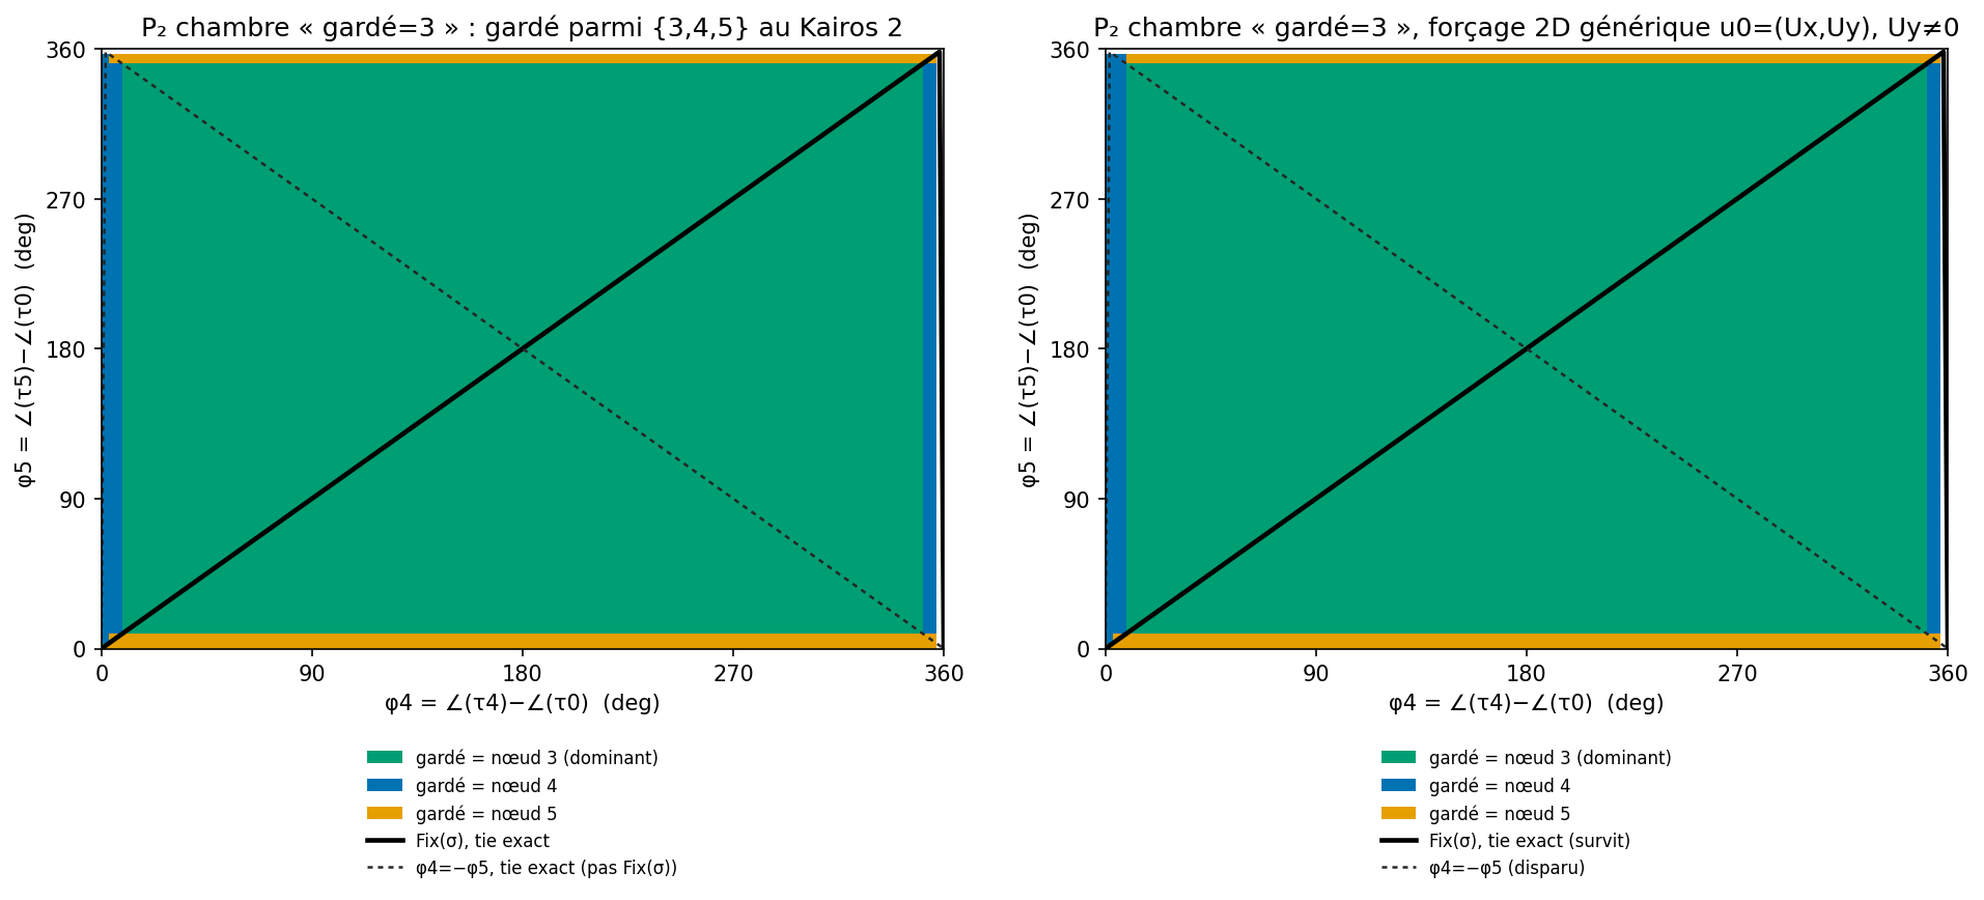
\includegraphics[width=\linewidth]{opacity_walls_protocol_control}
\caption{Témoin $N=6$ : séparation numérique entre une égalité de score portée par une symétrie effective et une égalité induite par le protocole. Le passage d'un forçage mono-axe à un forçage bidimensionnel générique conserve la diagonale structurelle et supprime l'antidiagonale protocolaire.}
\label{fig:opacity-walls-control}
\end{figure}

Une troisième situation apparaît dans la classe de mot où le premier recâblage garde le nœud $1$. On y vérifie
\[
\operatorname{Aut}(A_1)=\{e\}.
\]
Le recâblage suivant met pour la première fois les nœuds $4$ et $5$ en concurrence et fait apparaître deux bandes étroites. Ces bandes persistent sous le passage du forçage mono-axe au forçage bidimensionnel générique, mais leurs frontières se déplacent et se déforment. Comme aucune symétrie non triviale du graphe courant ne peut les porter et qu'elles ne disparaissent pas lorsque la symétrie accidentelle du protocole est cassée, elles fournissent ici des exemples numériques de coïncidences transverses de scores.

Ces trois diagnostics sont des outils d'analyse des expériences, et non une nouvelle taxonomie constitutive :
\[
\boxed{
\begin{array}{lll}
\text{symétrie effective de l'état} &:& \text{frontière exacte qui survit au contrôle},\\[1mm]
\text{symétrie du protocole} &:& \text{frontière qui disparaît sous une sonde générique},\\[1mm]
\text{coïncidence transverse} &:& \text{frontière qui subsiste mais se déforme.}
\end{array}}
\]

\subsection{Résolution, raffinement adaptatif et croissance locale sur $N=6$}

Un premier suivi global jusqu'à plusieurs Kairos, avec un forçage bidimensionnel générique, donnait à résolution $32\times32$ le comptage apparent
\[
3\longrightarrow3\longrightarrow5\longrightarrow5
\]
entre les profondeurs $k=2$ et $k=5$. Cette apparente stabilisation était toutefois un effet de sous-résolution. Un zoom local d'environ un facteur $20$ autour du coin $(0^\circ,0^\circ)$ révèle, à profondeur $k=4$, neuf chemins occupant tous des régions de taille substantielle : les quelques points isolés de la grille grossière étaient les traces sous-résolues de véritables classes locales.

Pour éviter de confondre longueur discrète de frontière et nombre géométrique de murs, les expériences notent
\[
N_{\partial,k}^{\mathrm{grid}}
\]
le nombre de transitions entre cellules voisines de la grille. Cette quantité dépend explicitement de la résolution et n'est utilisée que comme diagnostic numérique.

Une exploration adaptative a ensuite été appliquée sur tout le tore de la coupe $(\varphi_4,\varphi_5)$. Une grille grossière $16\times16$ est d'abord calculée ; seules les cellules dont les quatre coins ne portent pas la même étiquette de chemin sont ensuite raffinées par une grille locale $12\times12$. Dans l'expérience considérée, $60$ cellules sur $256$ sont ainsi raffinées. Elles se concentrent le long des frontières des deux bandes fines et dans leurs zones d'intersection.

\begin{figure}[H]
\centering
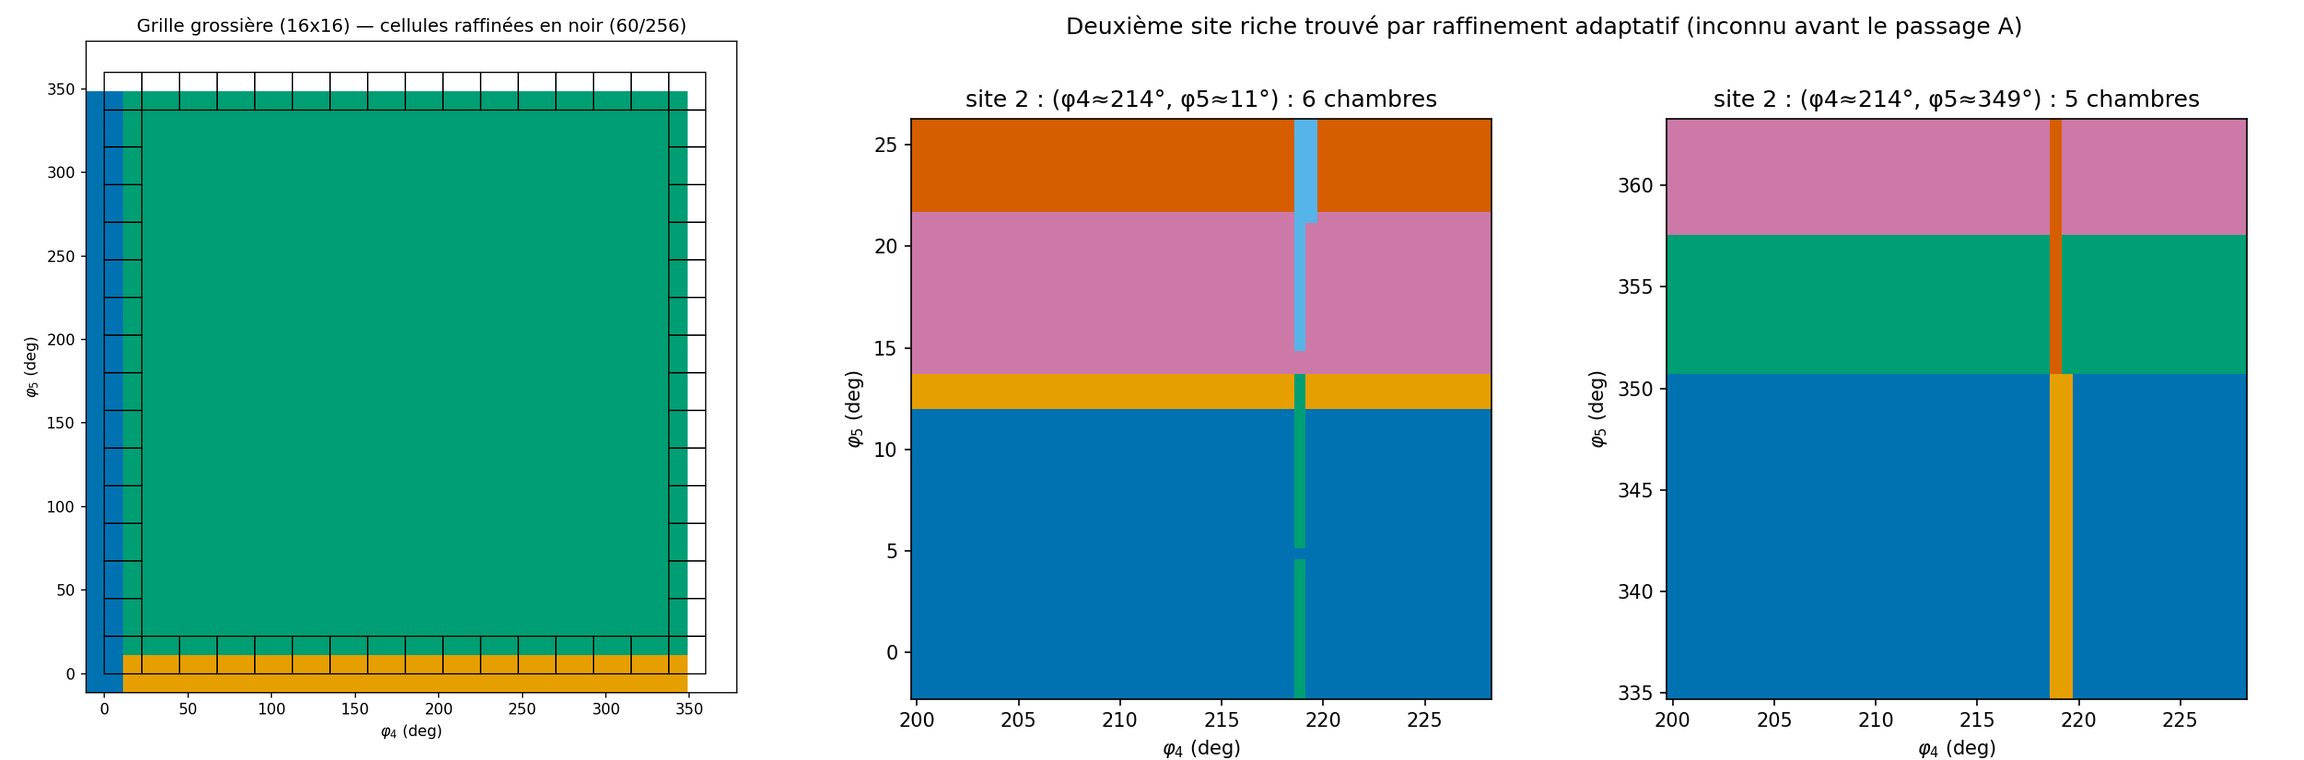
\includegraphics[width=\linewidth]{opacity_adaptive_refinement}
\caption{Exploration adaptative du témoin $N=6$. À gauche, les cellules de la grille grossière sélectionnées pour raffinement ; à droite, un second site localement riche révélé par cette stratégie.}
\label{fig:opacity-adaptive-refinement}
\end{figure}

Le motif de recompétition entre $4$ et $5$ n'est donc pas limité au coin initialement étudié : il réapparaît le long de ces frontières, avec une intensité variable. Le raffinement adaptatif fait également apparaître une seconde zone localement riche autour de $\varphi_4\simeq214^\circ$ et de deux valeurs complémentaires de $\varphi_5$. Cette seconde zone n'est pas encore expliquée par un mécanisme analytique ou combinatoire identifié ; elle reste un point de contrôle pour des travaux ultérieurs.

Ainsi, une grille uniforme peut donner une image qualitativement correcte de la partition tout en manquer des raffinements locaux. La complexité observée doit être rapportée avec la résolution et la stratégie d'échantillonnage utilisées.

\subsection{Un mécanisme local de réinjection combinatoire dans le témoin $N=6$}

Dans la seule zone située près de $(0^\circ,0^\circ)$, le suivi généalogique des classes de mot révèle un mécanisme plus précis. Chaque scission enregistrée conserve sa classe parente, les candidats en compétition et le diagnostic structurel ou transverse. Sur les branches effectivement explorées dans cette fenêtre, les profondeurs paires réactivent le même triplet compétitif
\[
\{1,4,5\}.
\]
Les profondeurs impaires ramènent le voisinage de $0$ dans un petit ensemble de configurations dont le recâblage suivant réinjecte ce même problème de classement. Numériquement, $\tau_1$ reste dans cette fenêtre le candidat dominant, de sorte que la compétition entre $4$ et $5$ est réouverte de manière récursive.

Le mécanisme combinatoire prédit alors, conditionnellement à la persistance de cette dominance, un arbre ternaire aux profondeurs paires : si $k=2n$,
\[
|\mathcal P_{2n}^{\mathrm{loc}}|=3^n
\]
au niveau de la règle génératrice. Numériquement, la grille raffinée résout $3$ classes de mot à $k=2$, $9$ à $k=4$ et $26$ à $k=6$, valeur compatible avec les $27$ branches idéales mais encore sensible à la résolution. Aucune nouvelle scission n'est observée entre $k=6$ et $k=7$ sur cette même grille.

\begin{figure}[H]
\centering
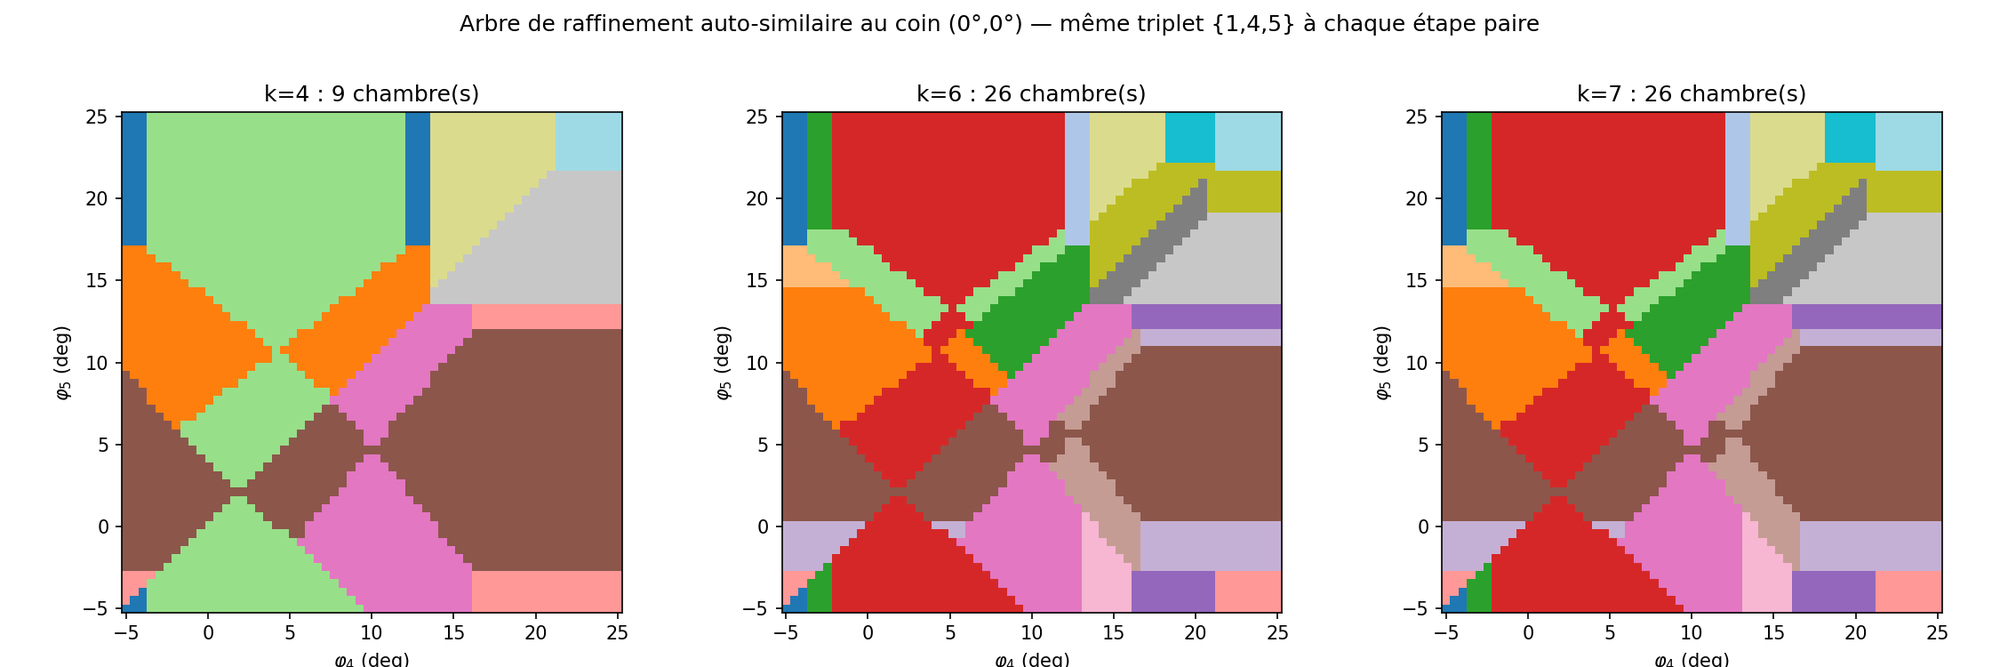
\includegraphics[width=\linewidth]{opacity_recursive_refinement}
\caption{Motif de raffinement récursif local du témoin $N=6$. Les panneaux montrent la même fenêtre aux profondeurs $k=4$, $k=6$ et $k=7$ ; la croissance du nombre de chemins est importante, mais organisée par une réinjection combinatoire identifiée.}
\label{fig:opacity-recursive-refinement}
\end{figure}

Il serait excessif d'en conclure à une auto-similarité globale du noyau IWS. Le mécanisme est établi ici uniquement pour ce site du témoin $N=6$ et pour le protocole étudié. Il convient en outre de distinguer deux niveaux de certitude : la récurrence des types de voisinages et des candidats est une propriété combinatoire vérifiée sur l'arbre de branches calculé ; la domination de $\tau_1$ sur toute une région continue reste, en l'absence d'une inégalité uniforme démontrée, un résultat numérique. Nous parlons donc seulement d'un \emph{motif de raffinement récursif local induit par une réinjection combinatoire}.

Ce cas montre que la croissance peut être non bornée, voire exponentielle en profondeur, tout en restant entièrement organisée par une règle locale simple. Ce qui est contrôlé n'est donc pas nécessairement le nombre de classes de mot, mais la structure de leur génération.

\subsection{Second témoin $N=9$ : hétérogénéité locale et réinjection structurelle}

Le témoin $N=9$ utilisé plus haut pour le crash-test du lemme orbital possède initialement
\[
N(0)=\{1,2,3\},
\qquad
N^c(0)=\{4,5\}\cup\{6,7,8\},
\qquad
|\operatorname{Aut}(A_0)|=72.
\]
Les voisins $\{1,2,3\}$ forment une orbite de taille $3$, tandis que les non-voisins se répartissent en orbites de tailles $2$ et $3$.

Sur une coupe générique $(\varphi_2,\varphi_6)$, la partition de profondeur un contient déjà quatre classes de mot :
\[
\{1,4,5\},\qquad
\{2,4,5\},\qquad
\{1,4,6\},\qquad
\{2,4,6\}.
\]
Une scission portée par l'échange des jumeaux $1$ et $2$ y coexiste dès le premier pas avec des scissions transverses impliquant le nœud $6$. Cette coexistence n'apparaissait qu'à profondeur supérieure sur le témoin $N=6$.

Les graphes postérieurs au premier Kairos présentent les diagnostics suivants :
\[
\begin{array}{c|c|c}
\text{classe de mot} & |\operatorname{Aut}(A_1)| & \text{orbites}\\
\hline
\{1,4,5\} & 240 & \{0\},\{1\},\{2,3,6,7,8\},\{4,5\}\\
\{2,4,5\} & 240 & \{0\},\{1,3,6,7,8\},\{2\},\{4,5\}\\
\{1,4,6\} & 48  & \{0\},\{1,6\},\{2,3,7,8\},\{4\},\{5\}\\
\{2,4,6\} & 48  & \{0\},\{1,3,7,8\},\{2,6\},\{4\},\{5\}
\end{array}
\]
Les deux premières structures sont isomorphes entre elles, de même que les deux dernières.

Une comparaison naïve sur la grille globale est biaisée par les aires très inégales des quatre classes. Un rééchantillonnage local à budget égal, avec $3600$ points appartenant effectivement à chaque classe à profondeur un, donne jusqu'à $k=5$ :
\[
\begin{array}{c|ccccc}
\text{classe} & k=1 & 2 & 3 & 4 & 5\\
\hline
\{1,4,5\} & 1&1&1&1&1\\
\{2,4,5\} & 1&2&2&3&3\\
\{1,4,6\} & 1&2&2&3&3\\
\{2,4,6\} & 1&3&3&6&6
\end{array}
\]
La classe la plus massive à profondeur un est localement la plus pauvre en profondeur, tandis que la classe marginale $\{2,4,6\}$ est la plus riche parmi les quatre zooms. Ni l'aire initiale, ni l'ordre du groupe d'automorphismes, ni la seule classe d'isomorphisme du graphe courant ne prédisent donc à eux seuls la richesse locale observée.

Un contrôle d'équivariance permet de séparer la structure du contexte caché. La transposition $\sigma=(1\ 2)$ appartient à $\operatorname{Aut}(A_0)$ et transporte $A_1^{\{1,4,5\}}$ sur $A_1^{\{2,4,5\}}$. En transportant également le point de zoom par $\sigma$, le calcul reproduit exactement la suite plate $1,1,1,1,1$ dans la classe transportée. La différence avec un autre centre de $\{2,4,5\}$ vient donc du contexte $\tau$, et non de l'étiquette des sommets.

La classe $\{2,4,6\}$ révèle en outre une réinjection structurelle spontanée. Au premier centre étudié, la suite locale jusqu'à $k=7$ est
\[
1,3,3,6,6,10,11.
\]
Toutes les scissions structurelles observées à $k=2$, $k=4$ et $k=6$ sont portées par la même transposition minimale
\[
(2\ 6),
\]
avec la même famille de quatre automorphismes témoins équivalents. Le mécanisme n'est pas attaché à une trajectoire unique : des branches ayant transité par des voisinages différents réactivent la même scission lorsqu'elles reviennent au voisinage $\{2,4,6\}$.

Un second point de zoom, choisi près du bord de l'arc continu correspondant à cette classe et sans rechercher une zone particulièrement riche, confirme le même mécanisme. La richesse numérique y est plus faible --- $1,2,2,4,4,5$ jusqu'à $k=6$ --- mais les scissions structurelles retrouvées à $k=4$ et $k=6$ portent encore exactement la même paire d'issues et le même témoin $(2\ 6)$. Cette robustesse est établie sur les deux régions explorées ; elle n'est pas promue ici en propriété uniforme démontrée de toute la classe.

Les deux témoins mettent ainsi en évidence deux mécanismes distincts de croissance organisée :
\[
\boxed{
\begin{array}{ll}
N=6:& \text{réinjection locale d'un même problème de classement,}\\[1mm]
N=9:& \text{réactivation d'une même symétrie au retour d'une configuration structurelle.}
\end{array}}
\]
Dans les deux cas, le simple nombre de classes de mot est moins informatif que la règle qui engendre leurs raffinements.


\subsection{De la profondeur finie à l'équivalence comportementale}

Les partitions expérimentales $\mathcal P_k$ ne sont utiles que si leur relation avec l'équivalence comportementale complète est explicitée. Pour une histoire commune $\mathcal H$ admissible depuis deux états $x,x'\in \mathcal O_y$, on note
\[
x\equiv_k^{\mathcal H}x'
\]
lorsque les deux exécutions produisent le même chemin structurel au cours de leurs $k$ premiers Kairos à granularité $G_1$. Si une exécution ou l'histoire considérée se termine avant le $k$-ième Kairos, ou si aucun Kairos supplémentaire ne survient, cette terminaison est incluse dans le préfixe observé ; elle ne peut donc être confondue avec une branche qui poursuit son chemin événementiel.

\begin{propositionthm}[Raffinement avec la profondeur]
Pour toute histoire $\mathcal H$ commune et tout $k\geq0$,
\[
\boxed{
 x\equiv_{k+1}^{\mathcal H}x'
 \quad\Longrightarrow\quad
 x\equiv_k^{\mathcal H}x'.}
\]
Par conséquent, pour un protocole fixé, $\mathcal P_{k+1}$ raffine $\mathcal P_k$.
\end{propositionthm}

\begin{proof}
Le chemin observé à profondeur $k$ est le préfixe de longueur $k$ du chemin observé à profondeur $k+1$. L'égalité de deux préfixes plus longs implique donc l'égalité de leurs préfixes plus courts.
\end{proof}

\begin{definition}[Équivalence comportementale de Nerode dans une fibre d'opacité]
Pour $x,x'\in \mathcal O_y$, on pose
\[
\boxed{
 x\sim_N x'
 \quad\Longleftrightarrow\quad
 \Madm_x=\Madm_{x'}
 \ \text{et}\ 
 R_x^{\rho_{\mathrm{int}}}=R_{x'}^{\rho_{\mathrm{int}}}}
\]
où l'égalité des applications de réponse est une égalité de fonctions, domaine compris.
\end{definition}

Dans le noyau découplé, l'équivalence de Nerode impose aussi l'accord des chemins structurels. En effet, si une histoire commune produisait une première divergence $A\neq A'$ au sortir d'un Kairos, la proposition d'identifiabilité structurelle montrerait que les deux états postérieurs ne peuvent pas avoir la même application de réponse $R^{\rho_{\mathrm{int}}}$. Par compatibilité préfixe--état, une continuation admissible distinguerait alors les deux réponses depuis les états initiaux, en contradiction avec $x\sim_Nx'$. Ainsi, dans ce régime, pour toute famille de protocoles $\mathcal U$,
\[
\boxed{
\sim_N\ \subseteq\
\bigcap_{\mathcal H\in\mathcal U}
\bigcap_{k<\infty}\equiv_k^{\mathcal H},}
\]
dès lors que les relations sont évaluées sur les histoires communes admissibles.

Dans le noyau, la clause de domaine peut elle aussi être vérifiée dans le régime maximal considéré ici. Le Volume I établit que toute condition initiale admissible et toute entrée mesurable essentiellement bornée engendrent une exécution hybride unique pour tout temps continu positif. Comme l'admissibilité initiale ne dépend que de $P$ et du graphe, deux états d'une même fibre $\mathcal O_y$, avec $y=(A,H,V,P)$, ont donc le même domaine maximal d'entrées bornées. Pour ce régime du noyau, $\Madm_x$ est ainsi constant sur $\mathcal O_y$.

\begin{propositionthm}[Complétude de la profondeur finie pour la famille maximale du noyau]
Dans le régime $\gamma_1=\lambda=0$ du noyau, pour la classe maximale des entrées mesurables essentiellement bornées et pour $x,x'\in \mathcal O_y$,
\[
\boxed{
 x\sim_Nx'
 \quad\Longleftrightarrow\quad
 \forall\mathcal H\in\Madm_x,\ \forall k<\infty,
 \quad x\equiv_k^{\mathcal H}x'.}
\]
\end{propositionthm}

\begin{proof}
Pour le sens direct, l'argument précédent exclut toute divergence structurelle sous une histoire commune : une telle divergence fournirait, par identifiabilité structurelle et compatibilité préfixe--état, une continuation qui contredirait $x\sim_Nx'$. On obtient donc $x\equiv_k^{\mathcal H}x'$ pour toute profondeur finie.

Pour la réciproque, fixons une histoire $\mathcal H$ et un horizon temporel fini $T$. Par absence de Zénon, l'exécution ne rencontre qu'un nombre fini de Kairos avant $T$. L'hypothèse d'accord à toute profondeur finie impose donc le même chemin structurel sur cet horizon. Par le lemme de constance du readout sur une chambre, les deux exécutions ont le même $(A,H,V,P)$ après chaque Kairos ; entre deux événements, elles suivent le même flot déterministe sous la même entrée. Leurs trajectoires $\rho_{\mathrm{int}}=(H,V,P)$ coïncident donc sur $[0,T]$. Comme $T$ est arbitraire, les réponses complètes coïncident sous $\mathcal H$. La constance du domaine admissible sur $\mathcal O_y$ donne la première clause de $\sim_N$.
\end{proof}

Ce résultat ne dit pas qu'une petite famille expérimentale suffit. Il déplace la question vers la réduction de la famille maximale.

\begin{definition}[Famille séparante]
Une famille $\mathcal U\subseteq\M$ est dite \emph{séparante} sur une fibre $\mathcal O_y$ si, pour toute paire $x,x'\in \mathcal O_y$ telle que $x\not\sim_Nx'$, il existe une histoire $\mathcal H\in\mathcal U$ et une profondeur finie $k$ qui distinguent la paire, soit par admissibilité, soit par
\[
x\not\equiv_k^{\mathcal H}x'.
\]
\end{definition}

La proposition précédente montre que la famille maximale est séparante dans le régime découplé. Le problème devient donc : jusqu'où peut-on réduire $\mathcal U$ sans perdre ce pouvoir ? Cette question est expérimentale avant de devenir un problème de minimalité analytique.

\subsection{Familles emboîtées de protocoles et transport de la différence cachée}

Les expériences utilisent notamment la chaîne suivante de familles du noyau :
\[
\mathcal U_5\subset\mathcal U_4\subset\mathcal U_3,
\]
où $\mathcal U_5$ contient les forçages constants mono-axe appliqués au nœud $0$, $\mathcal U_4$ les forçages constants bidimensionnels sur ce même nœud, et $\mathcal U_3$ les forçages constants bidimensionnels appliqués à un nœud arbitraire. Les calculs portent sur des échantillons finis emboîtés
\[
\widehat{\mathcal U}_5\subset\widehat{\mathcal U}_4\subset\widehat{\mathcal U}_3,
\]
qui ne doivent pas être confondus avec les familles mathématiques elles-mêmes. Un témoin positif de séparation est existentiel ; une absence de séparation sur un échantillon fini n'est pas une preuve d'impossibilité.

Sur trois paires de référence, avec le moteur numérique revalidé après correction et une profondeur de contrôle allant jusqu'à $k=12$ pour les absences observées, on obtient :
\[
\begin{array}{c|ccc}
\text{paire} & \mathcal U_5 & \mathcal U_4 & \mathcal U_3\\
\hline
A\ \text{-- miroir, }N=6 & \text{non séparée, preuve} & k_{\min}=3 & k_{\min}=1\\
B\ \text{-- coin, }N=6 & \text{non séparée observée} & k_{\min}=1 & k_{\min}=1\\
C\ \text{-- }\{2,4,6\},\ N=9 & \text{non séparée observée} & k_{\min}=2 & k_{\min}=2
\end{array}
\]
La paire miroir $A$ fournit une obstruction analytique à $\mathcal U_5$. Si $R_y$ désigne la réflexion de la seconde composante, le forçage mono-axe préserve le sous-espace $H_y=V_y=0$ et maintient les deux traces dans la relation miroir. Comme $R_y$ est orthogonale,
\[
\cos(R_ya,R_yb)=\cos(a,b),
\]
les classements de similarité restent identiques à chaque Kairos : $\mathcal U_5$ ne peut jamais séparer cette paire. Pour $B$ et $C$, aucune impossibilité analogue n'est établie ; les échecs de séparation rapportés restent des observations numériques.

\begin{lemma}[Transport de la différence cachée avant séparation]
Dans le régime $\gamma_1=\lambda=0$, considérons deux exécutions soumises à la même histoire et suivant le même chemin structurel sur un intervalle. Alors, pour tout nœud $j$,
\[
\Delta\tau_j(t)
= e^{-\beta(t-t_0)}\Delta\tau_j(t_0)
\]
tant que les deux exécutions n'ont pas divergé structurellement.
\end{lemma}

\begin{proof}
Tant que le chemin structurel est commun, les deux exécutions ont le même $A,H,V,P$. L'équation de trace du noyau est
\[
\dot\tau_j
=\alpha\tanh\!\bigl((\widetilde A H)_j\bigr)-\beta\tau_j.
\]
Le terme d'écriture est donc identique dans les deux exécutions et disparaît par soustraction :
\[
\Delta\dot\tau_j=-\beta\Delta\tau_j.
\]
Le saut de Kairos ne réinitialise pas $\tau$, de sorte que la relation se prolonge à travers les sauts communs tant qu'aucune divergence structurelle ne survient.
\end{proof}

Le protocole commun ne fabrique donc pas directement l'écart caché ; il déplace le fond commun relativement auquel $K^*$ lit cet écart. Numériquement, cette observation explique pourquoi la direction du contrôle peut être plus déterminante que son amplitude.

\subsection{Atteignabilité marginale et contrainte séquentielle}

Pour le témoin $N=9$ et la famille $\mathcal U_4$, on note $\theta_r(u)$ l'angle de $\tau_0$ au $r$-ième Kairos. Les balayages denses indiquent que la marginale de premier rang couvre numériquement tout le cercle : aucun arc interdit robuste ne subsiste lorsque la résolution angulaire est affinée. En revanche, l'ensemble conjoint
\[
\mathcal R_0^{(1,2)}(\mathcal U_4)
:=\{(\theta_1(u),\theta_2(u)):u\in\mathcal U_4\}
\subset S^1\times S^1
\]
reste fortement contraint. Sur une grille de $10^\circ$ et $4800$ protocoles, environ $86{,}3\%$ des cases du tore ne sont pas visitées, malgré la couverture complète des deux marginales. Un calcul de Jacobien montre une forte anisotropie : le déterminant relatif médian vaut environ $0{,}027$, avec de nombreuses zones presque dégénérées, mais des poches de rang plein subsistent. L'image n'est donc pas modélisée ici comme une courbe de rang un ; elle constitue plutôt un ensemble conjoint très plissé et fortement contraint.

\begin{figure}[H]
\centering
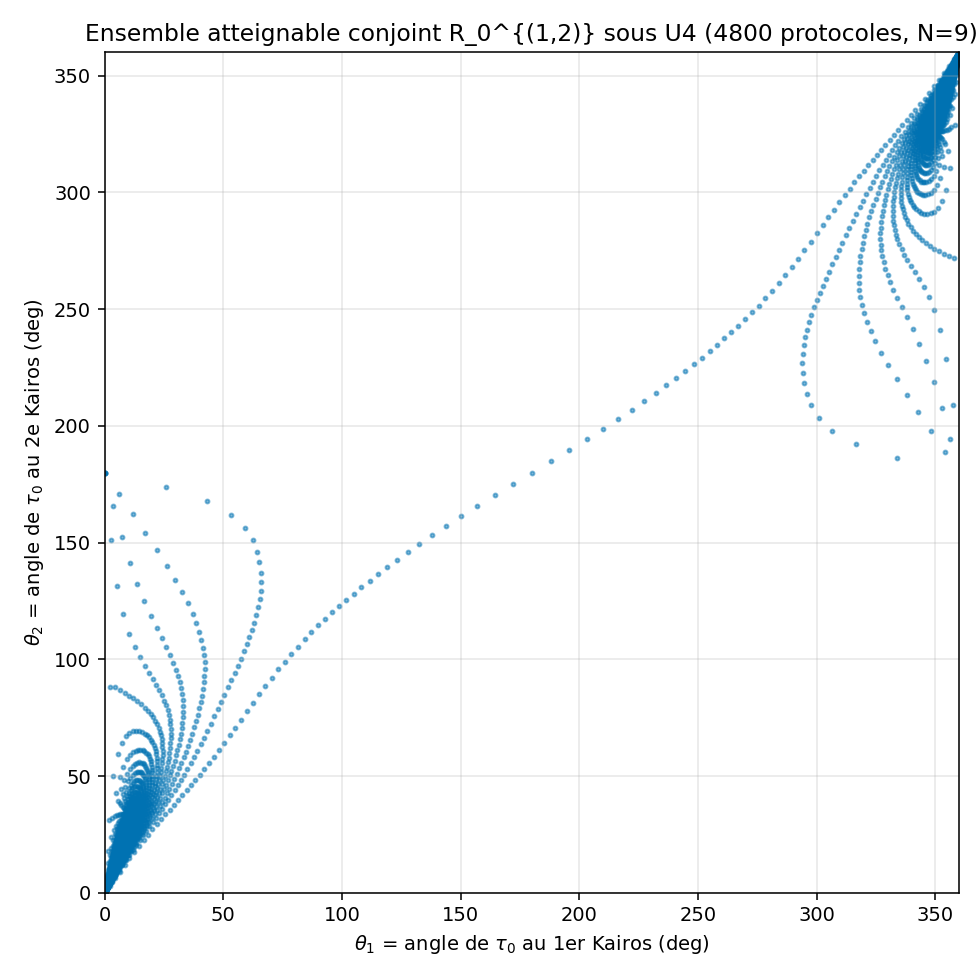
\includegraphics[width=0.82\linewidth]{reachability_joint_N9}
\caption{Témoin $N=9$ : ensemble conjoint numériquement atteignable des angles de $\tau_0$ aux deux premiers Kairos sous $\mathcal U_4$. Chaque marginale couvre le cercle à la résolution testée, alors que le conjoint reste fortement contraint. Ce résultat illustre la différence entre contrôlabilité marginale et contrôlabilité séquentielle.}
\label{fig:reachability-joint-n9}
\end{figure}

Cette expérience montre qu'une famille peut être riche à chaque étape considérée isolément tout en ne réalisant pas librement les successions correspondantes. La variable pertinente devient alors hybride : la structure intermédiaire $A_1$ conditionne les comparaisons disponibles au Kairos suivant. Les expériences conditionnées par classe de mot confirment ce point : pour une même paire cachée, certaines classes séparent fréquemment tandis que d'autres presque jamais, même lorsque les projections angulaires seules sont insuffisantes pour expliquer cette différence.

\subsection{Premier franchissement d'une marge de décision}

La projection angulaire reste néanmoins trop grossière pour identifier le mécanisme local de séparation. Considérons deux états d'une même fibre qui ne diffèrent initialement que par la trace d'un nœud $q$. Tant qu'ils suivent le même chemin structurel, le lemme précédent implique que toutes les traces $\tau_j$, $j\neq q$, restent identiques entre les deux exécutions. Au $r$-ième Kairos, supposons $q\neq i_r^*$, $m_r>0$ et aucune égalité exacte au seuil de sélection. Tous les scores autres que celui de $q$ sont alors identiques et déterminent un seuil commun.

On définit une marge signée $\operatorname{mar}_q^{(r)}$ positive lorsque $q$ est sélectionné par $K^*$ et négative lorsqu'il ne l'est pas : côté ajout, elle est le score de $q$ moins le seuil des $m_r$ meilleurs autres candidats ; côté retrait, elle est le seuil des $m_r$ plus faibles autres candidats moins le score de $q$.

\begin{propositionthm}[Premier franchissement de marge]
Sous les hypothèses précédentes, la première divergence structurelle des deux exécutions a lieu exactement au premier rang testable où les marges de sélection de $q$ ont des signes opposés. Hors tie exact,
\[
\boxed{
 k_{\min}
 =\min\Bigl\{r\geq1:
 \operatorname{mar}_q^{(r)}(x)\operatorname{mar}_q^{(r)}(x')<0\Bigr\}.}
\]
Les rangs où $m_r=0$ ne portent aucune décision compétitive et sont ignorés dans ce minimum.
\end{propositionthm}

\begin{proof}
Avant la première divergence, tous les candidats $j\neq q$ ont exactement les mêmes traces et les mêmes scores dans les deux exécutions ; le seuil pertinent est donc commun. Si les deux marges ont le même signe, $q$ a le même statut de sélection et, en l'absence de tie, l'ensemble complet des candidats sélectionnés est identique : le recâblage reste commun. Si les signes sont opposés, $q$ est sélectionné dans une exécution et pas dans l'autre ; comme la cardinalité sélectionnée est imposée, les deux ensembles d'arêtes modifiées diffèrent et les graphes post-Kairos divergent. L'argument s'itère jusqu'au premier changement de signe opposé.
\end{proof}

\begin{remark}
Le cas $q=i_r^*$ est exclu de l'énoncé : la trace perturbée devenant elle-même la référence des similarités, l'argument de seuil commun utilisé dans la preuve ne s'applique plus directement. Ce cas n'est pas rencontré dans l'expérience numérique rapportée ici et reste ouvert pour une extension ultérieure.
\end{remark}

Sur le témoin $N=9$ avec $q=7$, $800$ protocoles de $\mathcal U_4$ ont été poussés jusqu'à $K=7$. Parmi eux, $783$ rencontrent uniquement des rangs directement testables avant séparation : le premier flip de signe des marges reproduit $k_{\min}$ avec un accord exact de $100\%$, sans tie et sans que $q$ devienne lui-même déclencheur. Les $17$ autres rencontrent auparavant un Kairos avec $m_r=0$ ; ils restent non séparés jusqu'à $K=7$ et ne constituent pas des contre-exemples.

\begin{figure}[H]
\centering
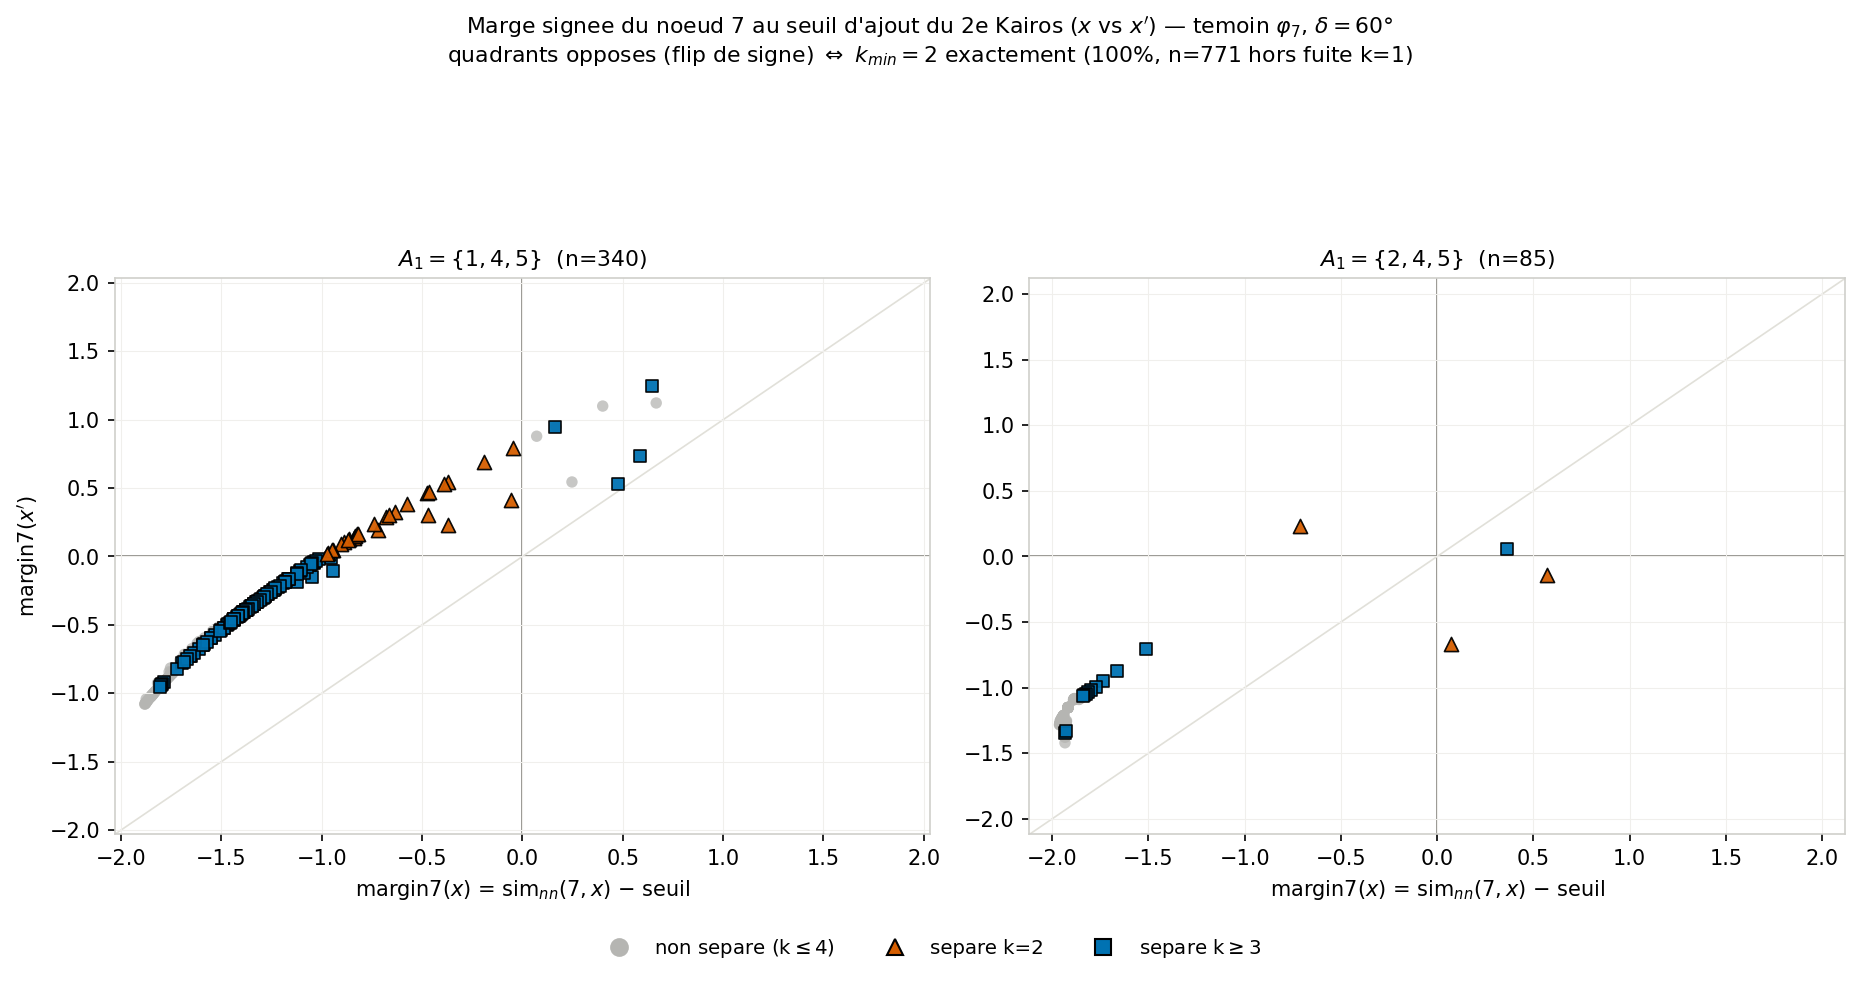
\includegraphics[width=0.92\linewidth]{margin_first_crossing_N9}
\caption{Cas illustratif $r=2$ pour le témoin $N=9$, paire ne différant que par $\tau_7$. Les quadrants opposés correspondent exactement à une divergence de signe de la marge. La validation numérique complète jusqu'à $K=7$ est donnée dans le texte.}
\label{fig:margin-first-crossing-n9}
\end{figure}

Ce résultat donne une lecture plus causale des partitions : dans ce cas, la profondeur de séparation est un temps de premier franchissement d'une surface de décision de $K^*$. Les angles et l'amplitude du protocole expliquent comment la trajectoire commune se déplace vers ces surfaces ; la marge en mesure directement la position pertinente pour la décision.

\subsection{Murs actifs et analyticité par morceaux}

Dans toute la suite de ce bloc, $k$ désigne la profondeur d'un mot ou d'une partition et $r$ le rang local d'un Kairos, avec $1\le r\le k$ ; au dernier Kairos d'un mot de longueur $k$, on a donc $r=k$.

Le critère de premier franchissement suggère de décrire directement les frontières des partitions par les égalités de scores qui peuvent modifier la sélection de $K^*$. Toutes les égalités $c_i=c_j$ ne sont toutefois pas pertinentes : si $i$ et $j$ sont simultanément sélectionnés, ou simultanément rejetés, leur permutation ne change pas le graphe post-Kairos. Seules les égalités situées à la coupure de la statistique d'ordre peuvent engendrer un nouveau mur.

Fixons une chambre $\Xi$ contenue dans une classe de mot de $\mathcal P_{k-1}$ et considérons le $k$-ième Kairos. On note $J_k^-$ l'ensemble des voisins candidats au retrait et $J_k^+$ l'ensemble des non-voisins candidats à l'ajout. Pour $j$ dans l'un de ces ensembles et $x\in\Xi$, on écrit
\[
 c_j^{(k)}(x)
 :=\cos\!\left(\tau_{i_k^*}^{(k)}(x),\tau_j^{(k)}(x)\right).
\]
Une paire $(i,j)$ est dite \emph{active au seuil} lorsqu'un échange de l'ordre de $c_i^{(k)}$ et $c_j^{(k)}$ peut modifier l'ensemble effectivement sélectionné par $K^*$ sur le côté considéré. On pose alors
\[
 W_{ij}^{(k)}(\Xi)
 :=\{x\in\Xi:c_i^{(k)}(x)=c_j^{(k)}(x)\}
 \cap\{(i,j)\text{ active au seuil}\}.
\]

Les dégénérescences propres au noyau sont regroupées dans
\[
\mathcal D_k
=
\underbrace{\{\dot P_{i_k^*}(t_k^*)=0\}}_{\text{contact tangent}}
\cup
\underbrace{\{\exists i\neq i_k^*:P_i(t_k^*)=\Theta\}}_{\text{Kairos simultané}}
\cup
\underbrace{\{\tau_{i_k^*}^{(k)}=0\ \text{ou}\ \exists j\in J_k^-\cup J_k^+:\tau_j^{(k)}=0\}}_{\text{formule analytique du cosinus non applicable}}.
\]

Dans le noyau du Volume I, la similarité est néanmoins définie par $s(i,j)=0$ si l'une des deux traces est nulle, et les égalités sont départagées déterministement par indice. Ainsi $\mathcal D_k$ signale ici la perte des hypothèses de la description analytique des murs, non un défaut de définition du saut. Le comptage semi-algébrique plus bas inclura ces lieux.

\begin{propositionthm}[Analyticité locale des scores et génération des murs]
Sur une sous-chambre d'une classe de $\mathcal P_{k-1}$ où le chemin combinatoire jusqu'au rang $k-1$ est fixé, supposons que le prochain Kairos soit unique et transverse, et que les vecteurs intervenant dans les cosinus restent non nuls. Alors le temps d'impact et l'état pré-Kairos dépendent analytiquement des données initiales tant que ces données influencent le flot analytiquement. Les scores $c_j^{(k)}$ sont donc analytiques par morceaux. Les coutures de leur statistique d'ordre sont portées par les égalités $c_i^{(k)}=c_j^{(k)}$ entre candidats.

En particulier,
\[
 \partial\mathcal P_k
 \subseteq
 \partial\mathcal P_{k-1}
 \cup
 \bigcup_{\Xi\in\pi_0(\mathcal P_{k-1})}
 \ \bigcup_{(i,j)\,\mathrm{actifs}}
 W_{ij}^{(k)}(\Xi)
 \cup
 \mathcal D_k,
\]
où $\pi_0(\mathcal P_{k-1})$ désigne la collection de toutes les composantes connexes des classes de mot de $\mathcal P_{k-1}$.
\end{propositionthm}

\begin{proof}
Le flot est analytique sur chaque région où les normes qui interviennent dans le champ restent non nulles. Si le contact avec le garde est défini localement par
\[
 P_{i_k^*}(t,x)-\Theta=0
\]
et si $\dot P_{i_k^*}(t_k^*)\neq0$, le théorème des fonctions implicites donne une dépendance analytique de $t_k^*$ en la donnée initiale $x$. La composition avec le flot puis avec la branche combinatoire fixée de $K^*$ conserve cette analyticité. Les cosinus sont analytiques hors vecteur nul. Enfin, sur une région où l'ordre des scores ne change pas, la statistique d'ordre est égale à l'un des scores analytiques ; elle ne change de formule que lorsqu'une égalité de scores est rencontrée. Une égalité interne au bloc sélectionné ou au bloc rejeté ne modifie pas $K^*$ ; seules les paires actives au seuil peuvent créer une frontière de la partition.
\end{proof}

Dans le régime découplé $\gamma_1=\lambda=0$ étudié ci-dessous, le résultat se simplifie encore : sur une classe de mot à readout fixé, $(H,V,P)$ et les temps de Kairos sont indépendants des coordonnées cachées. L'analyticité locale sera remplacée par une forme affine exacte de la trace.

\subsection{Murs transverses, murs forcés par symétrie et contrôle numérique}

Deux mécanismes doivent être distingués au niveau des composantes des zéro-sets. Pour
\[
 g_{ij}^{(r)}:=c_i^{(r)}-c_j^{(r)},
\]
une composante est \emph{transverse} lorsque
\[
 g_{ij}^{(r)}=0,
 \qquad
 \nabla g_{ij}^{(r)}\neq0.
\]
Elle est \emph{forcée par symétrie} lorsque l'annulation est identique sur une strate fixe d'une symétrie de la donnée pertinente pour l'opération courante, protocole compris. Une annulation avec gradient nul sans symétrie identifiée est conservée comme cas singulier ; elle n'est pas assimilée a priori à une symétrie.

Sur la fenêtre \texttt{site2\_bas} du témoin $N=6$, la superposition des murs actifs du quatrième Kairos à la partition observée donne un accord pixel à pixel de $100\%$ ($19600/19600$). La bande fine auparavant notée comme anomalie est entièrement reconstruite par deux composantes du même zéro-set
\[
 g_{14}^{(4)}=c_1^{(4)}-c_4^{(4)}=0.
\]
Sur la coupe $\varphi_5=349^\circ$, ses deux racines sont situées près de $218{,}56^\circ$ et $219{,}46^\circ$ ; elles sont transverses et de pentes opposées. Une même paire de scores peut donc produire plusieurs composantes de mur sans aucune dégénérescence.

\begin{figure}[H]
\centering
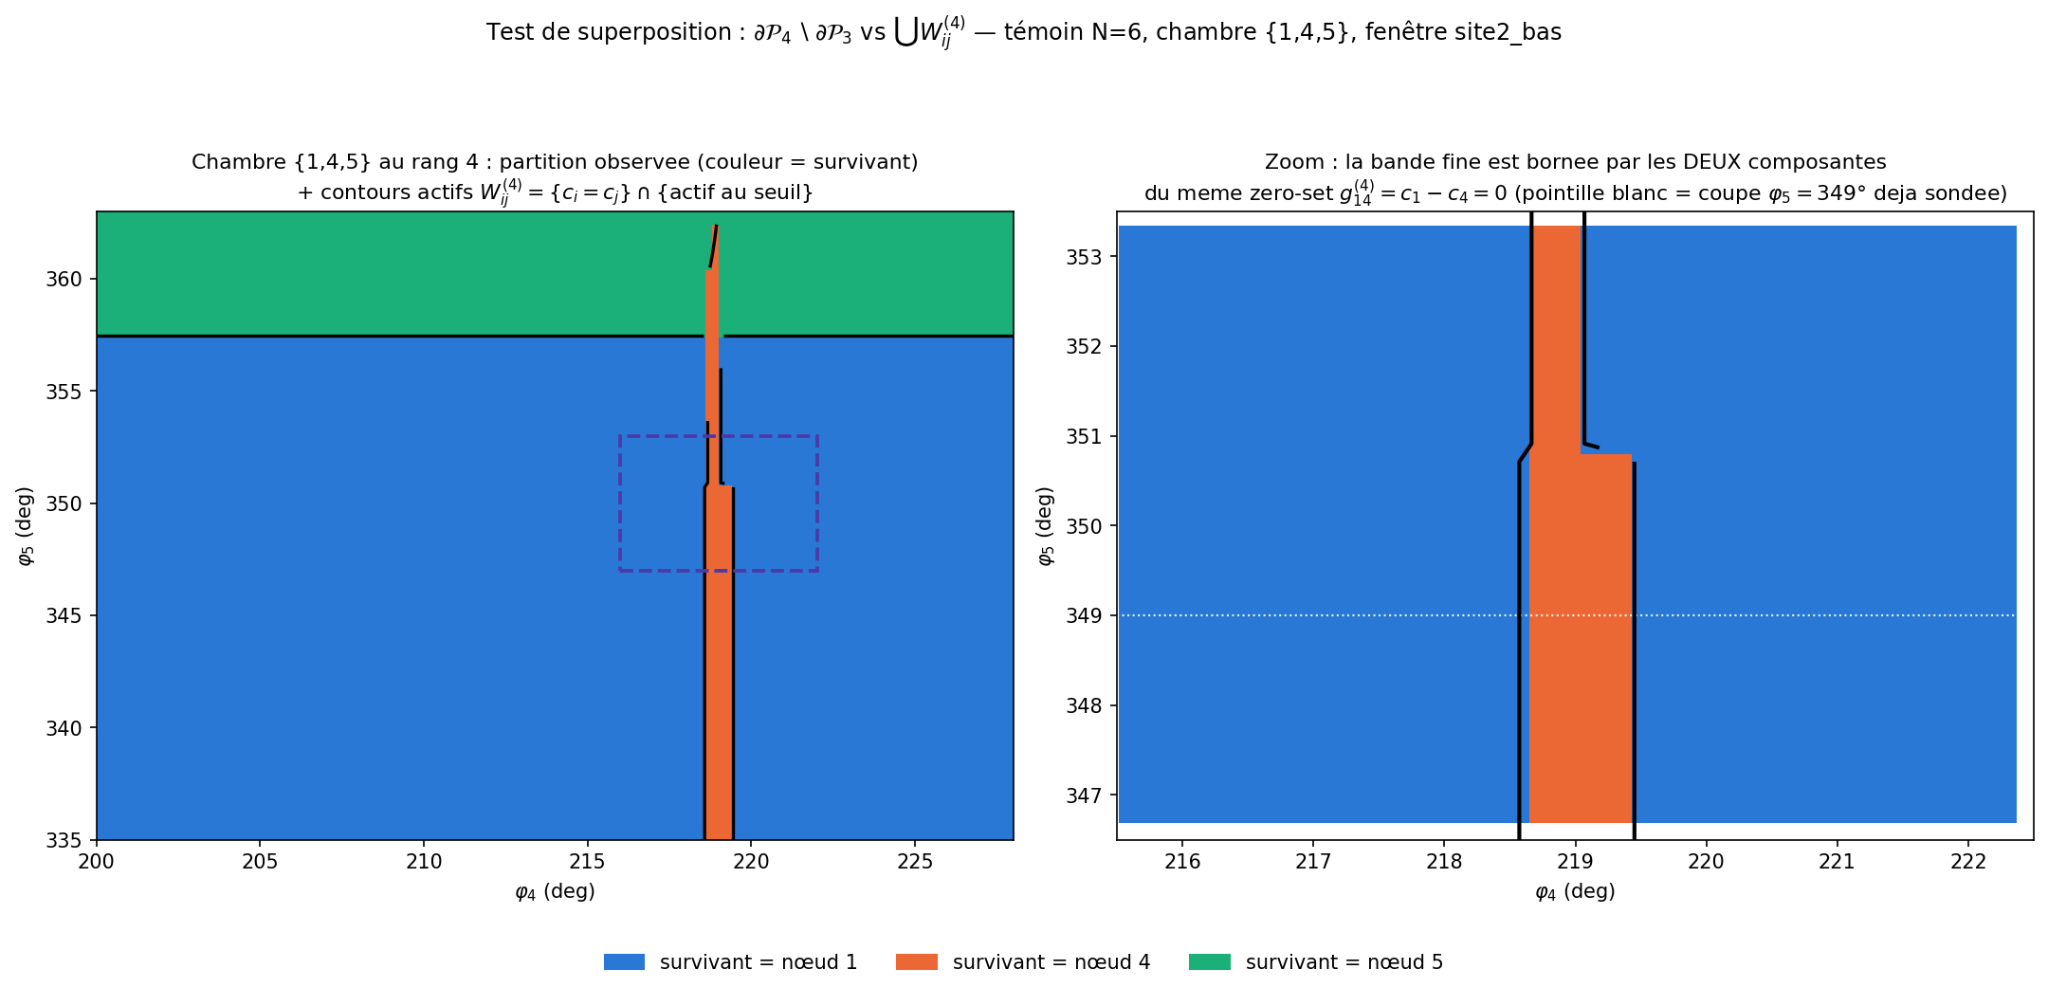
\includegraphics[width=\linewidth]{active_walls_site2_bas_r4}
\caption{Témoin $N=6$, fenêtre \texttt{site2\_bas} : superposition de la partition observée au rang $4$ et des zéro-sets des paires actives au seuil. Les contours reconstruisent exactement les frontières observées, y compris le doigt fin borné par deux composantes de $g_{14}^{(4)}=0$.}
\label{fig:active-walls-site2-r4}
\end{figure}

Le contrôle complémentaire est obtenu dans la classe de mot où une symétrie impose $\tau_1=\tau_2$. Au rang $2$, la composante structurelle de
\[
 W_{45}^{(2)}=\{c_4=c_5\}
\]
coïncide avec $\operatorname{Fix}(\sigma)$ pour $\sigma=(1\ 2)(4\ 5)$. Le long de cette diagonale,
\[
 \max|c_4-c_5|=1{,}08\times10^{-19},
\]
soit le niveau du bruit flottant. Hors de la diagonale, des branches transverses du même zéro-set subsistent. Les deux natures ne sont donc pas des propriétés exclusives d'une fonction $g_{ij}$ : elles peuvent appartenir à des composantes différentes de son zéro-set.

\begin{figure}[H]
\centering
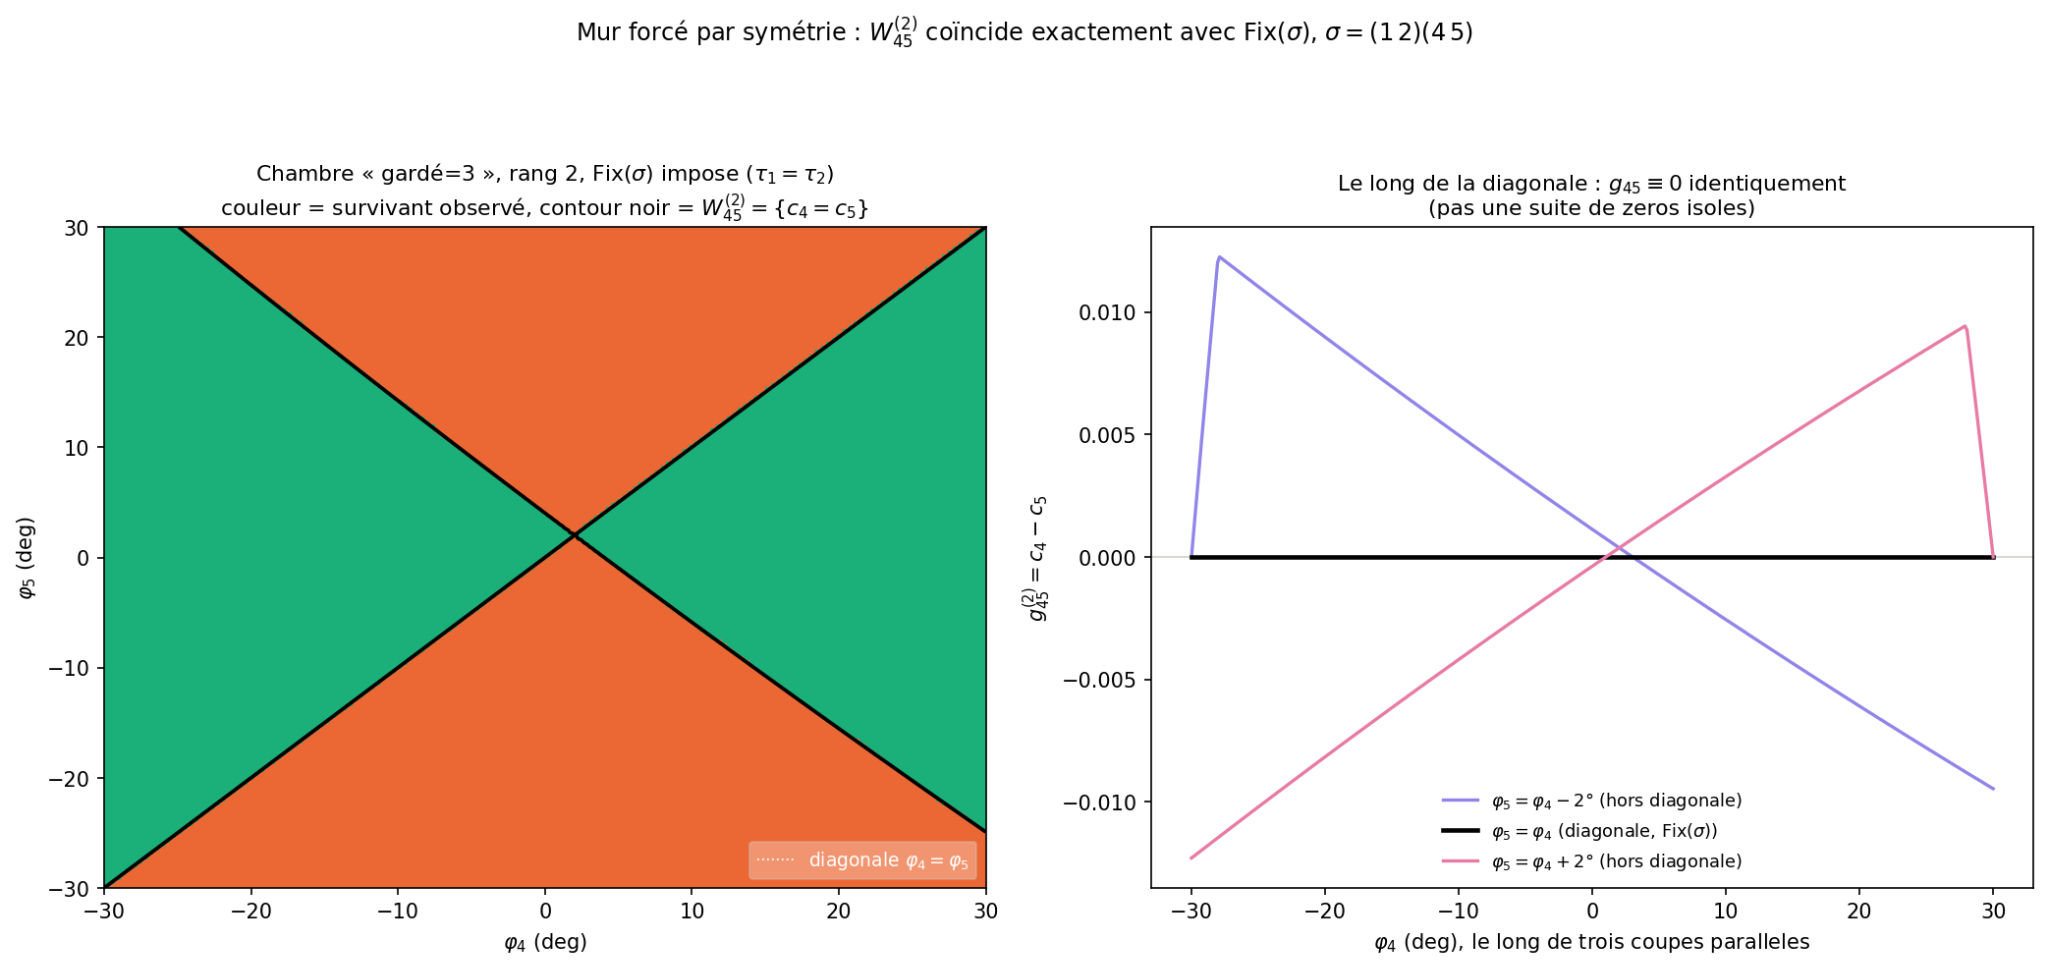
\includegraphics[width=\linewidth]{structural_wall_fixsigma}
\caption{Témoin $N=6$ : composante forcée par symétrie de $W_{45}^{(2)}$. Sur $\operatorname{Fix}(\sigma)$, $g_{45}^{(2)}$ s'annule identiquement à la précision machine ; sur deux coupes parallèles, l'annulation redevient isolée et transverse. Les désaccords bruts de classement sont confinés au tie exact, où la convention déterministe de départage attribue le mur à l'une des chambres.}
\label{fig:structural-wall-fixsigma}
\end{figure}

Ces deux contrôles montrent que l'extracteur de murs ne privilégie pas le cas générique : il retrouve aussi bien les croisements transverses que les composantes identiquement nulles imposées par une symétrie.

\subsection{Forme affine exacte de la trace à mot fixé}

Le régime découplé fournit un résultat plus fort que l'analyticité par morceaux.

\begin{lemma}[Forme affine exacte de la trace à mot fixé]
\label{lem:trace-affine-chambre}
Supposons $\gamma_1=\lambda=0$ et fixons un mot structurel $w$ dont le chemin $A_w(t)$ est commun à la classe considérée. Pour une coupe $\Sigma$ paramétrée par $\Phi:\Omega\to\Sigma$ comme ci-dessus, et pour les paramètres $\vartheta$ dont l'image réalise ce mot, on a, pour tout nœud $i$ et tout temps antérieur à la première divergence hors de ce mot commun,
\[
 \boxed{
 \tau_i(t;\vartheta)
 =b_{i,w}(t)+e^{-\beta t}\tau_i(0;\vartheta),}
\]
où
\[
 b_{i,w}(t)
 :=\alpha\int_0^t e^{-\beta(t-s)}
 \tanh\!\left((\widetilde A_w(s)H_w(s))_i\right)\,ds
\]
est indépendant de $\vartheta$. En particulier, au $r$-ième Kairos,
\[
 \tau_i^{(r)}(\vartheta)
 =b_{i,w}^{(r)}+\lambda_{r,w}\tau_i^0(\vartheta),
 \qquad
 \lambda_{r,w}=e^{-\beta t_{r,w}}.
\]
\end{lemma}

\begin{proof}
Dans le régime $\gamma_1=\lambda=0$, les équations de $(H,V,P)$ ne contiennent pas $\tau$. Sur une classe de mot où le chemin $A_w(t)$ est fixé, le déterminisme du flot impose donc les mêmes trajectoires $H_w,V_w,P_w$ pour tous les paramètres $\vartheta$ de la fibre. L'équation de trace
\[
 \dot\tau_i+\beta\tau_i
 =\alpha\tanh\!\left((\widetilde A_w H_w)_i\right)
\]
est linéaire avec second membre indépendant de $\vartheta$ ; la formule de variation des constantes donne l'identité annoncée. Le saut $K^*$ ne modifie pas $\tau$, de sorte que la formule traverse tous les Kairos communs.
\end{proof}

Cette identité a été contrôlée numériquement en ajustant $b$ et $\lambda$ sur deux points puis en évaluant tous les autres points de plusieurs chambres : les résidus maximaux observés sont $1{,}94\times10^{-16}$ et $1{,}55\times10^{-15}$, c'est-à-dire la précision machine attendue pour une identité exacte.

\begin{corollary}[Conservation du support de dépendance cachée]
Posons
\[
 \operatorname{Dep}(\Sigma):=\{i:\vartheta\mapsto\tau_i(0;\Phi(\vartheta))\text{ est non constante sur }\Omega\}.
\]
Tant que le chemin structurel reste commun, tout nœud extérieur à ce support reste gelé sur chaque réalisation du mot :
\[
 i\notin\operatorname{Dep}(\Sigma)
 \quad\Longrightarrow\quad
 \vartheta\mapsto\tau_i(t;\vartheta)\text{ est constante}.
\]
En particulier, une dépendance non constante observée sur une réalisation implique $i\in\operatorname{Dep}(\Sigma)$. La réciproque sur une réalisation particulière n'est pas affirmée sans hypothèse supplémentaire. Dans les familles affines considérées plus bas, si $\Omega$ est connexe et si $\vartheta\mapsto\tau_i^0(\Phi(\vartheta))$ est affine non constante sur $\Omega$, l'analyticité implique qu'elle ne peut être constante sur aucune partie relativement ouverte non vide de $\Omega$. Le support nodal de la dépendance paramétrique ne peut donc pas s'étendre d'un nœud à l'autre au fil des Kairos.
\end{corollary}

\begin{proof}
Si $i\notin\operatorname{Dep}(\Sigma)$, la donnée initiale $\tau_i(0;\vartheta)$ est indépendante de $\vartheta$ sur $\Omega$. Le terme $b_{i,w}(t)$ est lui aussi indépendant de $\vartheta$ et $e^{-\beta t}>0$ ; la formule affine du lemme montre donc que $\tau_i(t;\vartheta)$ reste constante sur toute réalisation du mot.
\end{proof}

Cette conservation induit une borne locale sur les comparaisons susceptibles de bouger. Au $r$-ième Kairos d'un mot de profondeur $k$, avec $1\le r\le k$, on note $J_r^-$ et $J_r^+$ les candidats au retrait et à l'ajout ; lorsque $r=k$, ils coïncident avec les ensembles $J_k^-$ et $J_k^+$ introduits plus haut. Pour $\varepsilon\in\{-,+\}$, posons
\[
 n_r^\varepsilon:=|J_r^\varepsilon|,
 \qquad
 \nu_r^\varepsilon:=|J_r^\varepsilon\cap\operatorname{Dep}(\Sigma)|.
\]

\begin{corollary}[Borne locale des comparaisons mobiles]
\label{cor:borne-paires-mobiles}
Supposons $i_r^*\notin\operatorname{Dep}(\Sigma)$. Sur le côté $\varepsilon\in\{-,+\}$, une comparaison $c_i^{(r)}-c_j^{(r)}$ ne peut dépendre de $\vartheta$ que si $\{i,j\}\cap\operatorname{Dep}(\Sigma)\neq\varnothing$. Si la sélection de cardinal $m_r$ est non triviale, le nombre de paires susceptibles d'être mobiles est donc borné par
\[
 \boxed{
 B_r^\varepsilon
 =\mathbf 1_{\{0<m_r<n_r^\varepsilon\}}
 \left[
 \nu_r^\varepsilon(n_r^\varepsilon-\nu_r^\varepsilon)
 +\binom{\nu_r^\varepsilon}{2}
 \right].}
\]
Pour $\nu_r^\varepsilon$ fixé, cette borne est linéaire en $n_r^\varepsilon$, et non quadratique.
\end{corollary}

\begin{proof}
Lorsque $i_r^*\notin\operatorname{Dep}(\Sigma)$, sa trace est indépendante de $\vartheta$. Tout candidat $j\notin\operatorname{Dep}(\Sigma)$ possède lui aussi une trace indépendante de $\vartheta$, donc un score constant dans la classe de mot. Une différence de scores ne peut être mobile que si au moins l'un des deux candidats appartient à $\operatorname{Dep}(\Sigma)$. Le nombre de telles paires est $\nu_r^\varepsilon(n_r^\varepsilon-\nu_r^\varepsilon)+\binom{\nu_r^\varepsilon}{2}$. Si $m_r=0$ ou $m_r=n_r^\varepsilon$, aucun classement compétitif n'est nécessaire.
\end{proof}

La condition $i_r^*\notin\operatorname{Dep}(\Sigma)$ est essentielle : si la trace du déclencheur varie elle-même, deux candidats hors de $\operatorname{Dep}(\Sigma)$ peuvent voir leurs deux scores varier par déplacement de la référence commune.

Sur le témoin $N=6$ étudié dans la fenêtre \texttt{site2\_bas}, $\operatorname{Dep}(\Sigma)=\{4,5\}$ et $i_r^*=0$ aux rangs considérés. L'alternance observée est portée non par l'ensemble total des candidats, constant, mais par le partage voisins/non-voisins. Aux rangs pairs $4$ et $6$, la réinjection ramène
\[
 J_r^-=\{1,4,5\},
\]
de sorte que les deux nœuds de $\operatorname{Dep}(\Sigma)$ sont simultanément engagés dans une sélection non triviale $3\to2$ ; des murs réapparaissent. Aux rangs impairs $5$ et $7$, le retrait contient soit aucun nœud de $\operatorname{Dep}(\Sigma)$, soit un seul nœud de $\operatorname{Dep}(\Sigma)$ isolé face à des candidats gelés ; aucun mur n'est observé dans la fenêtre.

Ce dernier point peut être fermé analytiquement au rang $5$. Dans un repère où la trace gelée du déclencheur donne l'axe horizontal, un nœud isolé de $\operatorname{Dep}(\Sigma)$ a une trace de la forme
\[
 \tau_{\mathrm{iso}}(\varphi)=b+a(\cos\varphi,\sin\varphi),
 \qquad b=(x,y),
\]
et son score est
\[
 c(\varphi)
 =\frac{x+a\cos\varphi}
 {\sqrt{(x+a\cos\varphi)^2+(y+a\sin\varphi)^2}}.
\]
Sa dérivée vaut
\[
 \boxed{
 c'(\varphi)
 =-\frac{a\,(y+a\sin\varphi)
 \bigl(a+x\cos\varphi+y\sin\varphi\bigr)}
 {\|\tau_{\mathrm{iso}}(\varphi)\|^3}.}
\]
Les points critiques sont donc parmi les solutions de
\[
 y+a\sin\varphi=0,
 \qquad
 a+x\cos\varphi+y\sin\varphi=0.
\]
Dans les deux chambres connexes impaires testées, aucune de ces solutions n'appartient à l'intervalle angulaire réel de la chambre. Le score isolé y est strictement monotone ; son minimum est atteint à une extrémité et reste strictement supérieur aux scores concurrents gelés. L'absence de mur est ainsi établie par un nombre fini d'évaluations aux extrémités, et non par un balayage de grille.

\subsection{Réduction semi-algébrique à mot structurel fixé}

La forme affine précédente permet de remplacer la question d'une complexification analytique locale par une question de géométrie semi-algébrique, pour les familles cachées paramétrées algébriquement. On suppose désormais que le domaine de paramètres $\Omega$ introduit plus haut est une partie semi-algébrique fixée de
\[
 (S^1)^p\subset\mathbb R^{2p},
\]
par exemple $(S^1)^p$ lui-même ou un produit fini d'arcs semi-algébriques correspondant à une boîte angulaire. La paramétrisation $\Phi:\Omega\to\Sigma$ est supposée être un homéomorphisme sur son image. On tire en arrière les classes de $\mathcal P_k(\Sigma)$ par $\Phi$ ; comme $\Phi$ est un homéomorphisme, ce passage conserve exactement les composantes connexes. Dans cette sous-section, on conserve par abus la notation $\mathcal P_k$ pour cette partition tirée en arrière.

On écrit
\[
 z=(z_1,\dots,z_p)\in\Omega,
 \qquad
 z_\ell=(x_\ell,y_\ell),
 \qquad
 x_\ell^2+y_\ell^2=1,
\]
et l'on suppose que les traces initiales dépendent affinement de $z$. Le vecteur $z$ fournit ainsi les coordonnées algébriques du paramètre caché $\vartheta\in\Omega$. C'est notamment le cas des familles angulaires utilisées dans les témoins numériques, avec normes initiales fixées.

Fixons une profondeur $k$ et un mot structurel $w$ de longueur $k$. Pour tout rang local $1\le r\le k$, le lemme~\ref{lem:trace-affine-chambre} donne, sur toute réalisation de $w$,
\[
 \tau_i^{(r)}(z)=b_{i,w}^{(r)}+\lambda_{r,w}\tau_i^0(z),
\]
donc une dépendance affine en $z$. Les quantités $b_{i,w}^{(r)}$ et $\lambda_{r,w}$ peuvent contenir les intégrales et fonctions transcendantes du flot, mais elles sont constantes par rapport à $z$ une fois le mot $w$ fixé : dans le régime découplé, un même mot impose le même chemin $A_w$, donc les mêmes trajectoires $(H,V,P)$ et les mêmes temps de Kairos. Elles jouent ainsi le rôle de coefficients réels dans les équations qui suivent, indépendamment de la composante connexe particulière réalisant $w$.

Écrivons directement
\[
 \tau_\star:=\tau_{i_r^*}^{(r)}(z),
 \qquad
 a_i:=\langle \tau_\star,\tau_i^{(r)}(z)\rangle,
 \qquad
 s_i:=\|\tau_i^{(r)}(z)\|^2.
\]
Sur le lieu régulier $\|\tau_\star\|>0$, $s_i>0$, l'égalité de deux cosinus s'écrit
\[
 \frac{a_i}{\sqrt{s_i}}
 =\frac{a_j}{\sqrt{s_j}}.
\]
Elle est exactement équivalente à la condition semi-algébrique
\[
 \boxed{
 a_i^2s_j-a_j^2s_i=0,
 \qquad
 a_ia_j\ge0.}
\]
La seconde condition restaure le signe perdu par l'élévation au carré et élimine en particulier la branche parasite $c_i=-c_j$.

Les inégalités de classement sont elles aussi semi-algébriques. En posant
\[
 \chi_{ij}:=a_i^2s_j-a_j^2s_i,
\]
la relation $c_i\ge c_j$ est, sur le lieu régulier, la réunion des trois cas
\[
 \begin{aligned}
 &a_i\ge0>a_j,\\
 &a_i\ge0,\ a_j\ge0,\ \chi_{ij}\ge0,\\
 &a_i<0,\ a_j<0,\ \chi_{ij}\le0.
 \end{aligned}
\]
Une réalisation complète d'un classement est donc une combinaison booléenne finie de conditions polynomiales.

Deux régimes de degré doivent être distingués. Si $i_r^*\notin\operatorname{Dep}(\Sigma)$, alors $\tau_\star$ est constant sur la famille paramétrée :
\[
 \deg a_i\le1,
 \qquad
 \deg s_i\le2,
 \qquad
 \deg \chi_{ij}\le4,
 \qquad
 \deg(a_ia_j)\le2.
\]
Si $i_r^*\in\operatorname{Dep}(\Sigma)$, $\tau_\star$ est lui-même affine en $z$ :
\[
 \deg a_i\le2,
 \qquad
 \deg s_i\le2,
 \qquad
 \deg \chi_{ij}\le6,
 \qquad
 \deg(a_ia_j)\le4.
\]
Ainsi, dans les deux cas,
\[
 \boxed{\deg\le6}
\]
suffit uniformément pour les polynômes qui déterminent les murs et les comparaisons, indépendamment de la profondeur $k$. La profondeur change les coefficients rencontrés et la combinatoire des classements successifs, pas le degré local des frontières.

\subsection{Borne de croissance des chambres, ties inclus}

On conserve le régime découplé $\gamma_1=\lambda=0$, une lecture initiale $y$ et un protocole fixés, un nombre $N$ de nœuds fixé, ainsi que le domaine semi-algébrique $\Omega\subset(S^1)^p$ et l'homéomorphisme $\Phi:\Omega\to\Sigma$. On suppose les $k$ premiers Kairos définis pour les exécutions considérées. Les mots $w$ sont ici \emph{complets pour la décision} : outre les structures post-cascade, ils identifient les étapes de cascade simultanée nécessaires pour déterminer le chemin visible et les coefficients $b_{i,w}^{(r)},\lambda_{r,w}$. La convention déterministe du Volume I (priorité au saut, plus petit indice, puis départage par indice des égalités de scores) est conservée, y compris lorsque plusieurs Kairos se produisent simultanément.

Pour chaque préfixe de $w$ et chaque rang $1\le r\le k$, les coefficients de la forme affine sont constants en $z$. On considère les polynômes
\[
 a_i^{(r)}=\langle\tau_\star^{(r)},\tau_i^{(r)}\rangle,\qquad
 s_i^{(r)}=\|\tau_i^{(r)}\|^2,\qquad
 \chi_{ij}^{(r)}=(a_i^{(r)})^2s_j^{(r)}-(a_j^{(r)})^2s_i^{(r)},
\]
ainsi que $s_\star^{(r)}=\|\tau_\star^{(r)}\|^2$. Leurs degrés ne dépassent pas $6$. La famille des polynômes intervenant dans les classements successifs, notée $\mathscr F_w$, a une cardinalité au plus $B_N k$ pour une constante $B_N$ dépendant de $N$ et du codage choisi des macrocascades. On ajoute à cette famille les contraintes fixes définissant $\Omega$.

\begin{lemma}[Le vecteur de signes détermine la décision]
\label{lem:signes-determinent-kstar}
Dans une branche à chemin visible fixé, le vecteur des signes $(-,0,+)$ des polynômes de $\mathscr F_w$ détermine entièrement le préordre des scores de similarité utilisés par $K^*$, y compris lorsque certaines traces sont nulles. Le départage déterministe en déduit un ensemble sélectionné unique.
\end{lemma}
\begin{proof}
Si $s_\star^{(r)}=0$ ou $s_i^{(r)}=0$, le score correspondant est $0$ par la règle du noyau, ce que détectent les signes des polynômes quadratiques. Sinon, le signe de $a_i^{(r)}$ est celui de $c_i^{(r)}$. Pour deux scores strictement positifs, le signe de $c_i^{(r)}-c_j^{(r)}$ est celui de $\chi_{ij}^{(r)}$ ; pour deux scores strictement négatifs, il est opposé. Les signes opposés et les cas où un score est nul sont directement ordonnés par les signes de $a_i^{(r)}$, $a_j^{(r)}$, $s_i^{(r)}$, $s_j^{(r)}$ et $s_\star^{(r)}$. Les égalités exactes sont détectées et départagées par indice. Toutes les comparaisons et la sélection sont donc fonctions du vecteur de signes.
\end{proof}

La réalisation $\Omega_w$ d'un mot $w$ n'est généralement \emph{pas une unique} réalisation de signes : elle est une \emph{réunion} de telles réalisations, celles pour lesquelles toutes les décisions successives redonnent $w$. En particulier, la relation $c_i\ge c_j$ correspond à une combinaison booléenne de conditions de signes et non à une condition de signe unique. Les lieux de ties, y compris les composantes de codimension positive, appartiennent aux réalisations ainsi définies.

\begin{propositionthm}[Complexité semi-algébrique à mot fixé, ties inclus]
\label{prop:complexite-mot-fixe}
Sous les hypothèses précédentes, et pour $p,N$ fixés, il existe une constante $B_{\mathrm{sa}}>0$, indépendante de $k$ et du mot réalisable $w$, telle que
\[
 \boxed{b_0(\Omega_w)\le B_{\mathrm{sa}}\,k^p.}
\]
La borne inclut les départages exacts et les lieux où une trace s'annule.
\end{propositionthm}
\begin{proof}
Les réalisations des conditions de signes de $\mathscr F_w$ sont semi-algébriques sur $\Omega$. Le théorème de Barone--Basu sur le nombre total de composantes semi-algébriquement connexes de \emph{toutes} les réalisations de conditions de signes sur une variété algébrique réelle de dimension $p$ donne ici $O((B_Nk)^p)$, à degrés et dimension ambiante fixés. Les contraintes semi-algébriques fixes de $\Omega$ sont incorporées dans la famille de signes sans faire dépendre leur nombre de $k$. Puisque $\Omega_w$ est une réunion de certaines de ces cellules de signes, son nombre de composantes ne dépasse pas la somme des nombres de composantes des cellules retenues. On obtient la borne annoncée. Voir S.~Barone et S.~Basu, \emph{Refined bounds on the number of connected components of sign conditions on a variety}, Discrete \& Computational Geometry 47 (2012), 577--597, DOI: \href{https://doi.org/10.1007/s00454-011-9391-3}{10.1007/s00454-011-9391-3} ; voir aussi Basu--Pollack--Roy, \emph{Algorithms in Real Algebraic Geometry}, chap.~7 pour les outils généraux de conditions de signes.
\end{proof}

Chaque paramètre de $\Omega$ réalise un unique mot complet de profondeur $k$, dès lors que cette profondeur est atteinte, car les ties et les cascades sont résolus par la sémantique du noyau. Si $\mathcal W_k$ désigne les mots ainsi réalisables, nous avons donc \emph{exactement}
\[
 \boxed{\Omega=\bigsqcup_{w\in\mathcal W_k}\Omega_w.}
\]
On appelle $\mathcal P_k^{\mathrm{conn}}$ l'ensemble des composantes connexes de toutes ces classes de mot (après tirage en arrière par $\Phi$). Le décompte topologique est alors
\[
 \boxed{ |\mathcal P_k^{\mathrm{conn}}|=\sum_{w\in\mathcal W_k} b_0(\Omega_w).}
\]
À $N$ fixé, le nombre d'issues possibles d'une macrocascade est majoré par une constante finie $L$ ; il en résulte $|\mathcal W_k|\le L^k$ pour les mots atteignant la profondeur $k$.
\begin{corollary}[Borne de croissance des chambres, ties inclus]
\label{cor:borne-croissance-ties}
Il existe $B_{\mathrm{conn}}>0$, indépendant de $k$, tel que
\[
 \boxed{|\mathcal P_k^{\mathrm{conn}}|\le B_{\mathrm{conn}}\,k^pL^k.}
\]
Si certaines exécutions n'atteignent pas le $k$-ième Kairos, l'énoncé s'applique au domaine des exécutions qui l'atteignent. Une extension à tous les points demande un codage explicite des mots tronqués et des domaines correspondants.
\end{corollary}

Cette borne est une borne de \emph{comptage}. Elle n'impose ni transversalité des Kairos, ni absence de traces nulles ou de ties. En revanche, la description des \emph{frontières comme murs analytiques} dans la proposition précédente reste limitée à ses hypothèses de régularité : la règle de score nul, bien définie, n'est pas continue au travers d'une annulation de trace.

\subsection{Bifurcation conique lorsque la trace s'annule}

Pour étudier la variation du présent observable, faisons dépendre une composante initiale visible de $y$ d'un paramètre réel $\mu$, sans modifier le protocole ni la coupe cachée. Au voisinage d'une région où le préfixe événementiel est fixé, la forme affine donne, pour un nœud $j$ et une coordonnée angulaire $\varphi$,
\[
 \tau_j^{(r)}(\varphi,\mu)
 =b_{j,w}^{(r)}(\mu)+R_j(\mu)e(\varphi),\qquad
 e(\varphi)=(\cos\varphi,\sin\varphi),\quad R_j(\mu)>0.
\]
Ici $b_{j,w}^{(r)}(\mu)$ est le terme de translation associé au chemin visible $w$, et $R_j(\mu)=\lambda_{r,w}(\mu)\rho_j$ lorsque la trace initiale angulaire du nœud $j$ a une norme fixe $\rho_j>0$. Le cercle complet correspondant rencontre l'origine si et seulement si
\[
 \boxed{\Delta_{j,w}^{(r)}(\mu)
 :=\bigl\|b_{j,w}^{(r)}(\mu)\bigr\|^2-R_j(\mu)^2=0.}
\]
Une racine $\mu_*$ ne produit une annulation dans le \emph{domaine du préfixe considéré} que si $\varphi_*:=\arg\!\bigl(-b_{j,w}^{(r)}(\mu_*)\bigr)$ y est admissible. On note $\mathcal V_{w^-}$ la région du plan $(\varphi,\mu)$ où le préfixe événementiel $w^-$, antérieur au saut étudié, est réalisé ; la décision au saut suivant n'est pas fixée dans $\mathcal V_{w^-}$.

\begin{propositionthm}[Forme normale conique d'une annulation transverse]
\label{prop:annulation-conique}
Supposons $b_{j,w}^{(r)}$ et $R_j$ de classe $C^2$ près de $\mu_*$, et posons $\varphi_*=\arg\!\bigl(-b_{j,w}^{(r)}(\mu_*)\bigr)$. Supposons
\[
 \Delta_{j,w}^{(r)}(\mu_*)=0,\qquad
 \bigl(\Delta_{j,w}^{(r)}\bigr)'(\mu_*)\ne0,\qquad
 (\varphi_*,\mu_*)\in\operatorname{int}(\mathcal V_{w^-}).
\]
Alors l'application $\Psi_j:(\varphi,\mu)\mapsto\tau_j^{(r)}(\varphi,\mu)$ est un difféomorphisme local en $(\varphi_*,\mu_*)$. Plus précisément, pour $\varphi$ en radians,
\[
 \boxed{\bigl(\Delta_{j,w}^{(r)}\bigr)'(\mu_*)=
 2\det\bigl[\partial_\varphi\Psi_j,\partial_\mu\Psi_j\bigr]_{(\varphi_*,\mu_*)}.}
\]
Supposons en outre que la trace de référence $\tau_\star(\mu)$ soit de classe $C^1$ et non nulle près de $\mu_*$, et que le seuil concurrent $c_{\mathrm{seuil}}(\mu)$ soit de classe $C^1$ et vérifie $0<c_{\mathrm{seuil}}(\mu_*)<1$. Pour cette proposition locale, ces deux quantités sont supposées indépendantes de $\varphi$ à préfixe fixé. Dans le plan de $\Psi_j$, soient $\theta_\pm^*$ les deux directions limites du secteur $c_j>c_{\mathrm{seuil}}$ ; on suppose que ces directions sont transverses aux coupes $\mu=\mathrm{constante}$ et qu'elles rencontrent ces coupes du même côté de $\mu_*$. Alors, de ce côté, les deux frontières actives issues de l'annulation possèdent un écart angulaire
\[
 \boxed{L(\mu)=\upsilon_{\mathrm{cone}}|\mu-\mu_*|
 +o(|\mu-\mu_*|),\qquad \upsilon_{\mathrm{cone}}>0,}
\]
avec la formule explicite de $\upsilon_{\mathrm{cone}}$ donnée dans la preuve. Cette proposition est locale et ne garantit ni la présence ni l'absence d'autres régions de sélection ailleurs sur le cercle.
\end{propositionthm}
\begin{proof}
Écrivons pour alléger $b(\mu)=b_{j,w}^{(r)}(\mu)$ et $R(\mu)=R_j(\mu)$. À l'annulation, $b(\mu_*)=-R(\mu_*)e(\varphi_*)$. Avec $e^\perp=(-\sin\varphi,\cos\varphi)$, nous avons
\[
 \partial_\varphi\Psi_j=R e^\perp,
 \qquad \partial_\mu\Psi_j=b'+R'e.
\]
D'où, au point critique,
\[
 \bigl(\Delta_{j,w}^{(r)}\bigr)'
 =2\langle b,b'\rangle-2RR'
 =-2R\bigl(\langle e,b'\rangle+R'\bigr)
 =2\det[Re^\perp,b'+R'e].
\]
La dérivée non nulle permet d'appliquer le théorème d'inversion locale à $\Psi_j$. Notons
\[
 J:=D_{(\varphi,\mu)}\Psi_j(\varphi_*,\mu_*),
 \qquad \mathbf e(\theta):=(\cos\theta,\sin\theta).
\]
Dans le plan image, introduisons les coordonnées polaires $\Psi_j=\rho\,\mathbf e(\theta)$, $\rho>0$. Le développement $C^2$ de l'inverse du difféomorphisme local donne, en posant $\xi=\varphi-\varphi_*$ et $\epsilon=\mu-\mu_*$,
\[
 \begin{split}
 \xi&=\rho\,m(\theta)+O(\rho^2),\\
 \epsilon&=\rho\,\ell(\theta)+O(\rho^2),
 \end{split}
 \qquad
 \begin{cases}
 m(\theta)=\operatorname{pr}_1\!\bigl(J^{-1}\mathbf e(\theta)\bigr),\\
 \ell(\theta)=\operatorname{pr}_2\!\bigl(J^{-1}\mathbf e(\theta)\bigr).
 \end{cases}
\]
Hors de l'origine, la frontière de sélection $c_j=c_{\mathrm{seuil}}$ s'écrit en coordonnées polaires
\[
 \theta=\theta_\pm(\mu)
 :=\arg\widehat\tau_\star(\mu)
 \pm\arccos\bigl(c_{\mathrm{seuil}}(\mu)\bigr),
 \qquad \theta_\pm^*=\theta_\pm(\mu_*).
\]
Ces deux directions sont distinctes puisque $0<c_{\mathrm{seuil}}(\mu_*)<1$. La fonction angulaire n'est \emph{pas} différentiable à $\Psi_j=0$ : on n'y applique donc pas le théorème des fonctions implicites. Les hypothèses de transversalité sont précisément
\[
 \ell_\pm:=\ell(\theta_\pm^*)\ne0,
 \qquad \operatorname{sign}(\ell_+)=\operatorname{sign}(\ell_-).
\]
Sur le côté $\operatorname{sign}(\epsilon)=\operatorname{sign}(\ell_\pm)$, on applique séparément le théorème des fonctions implicites dans les variables $(\rho,\epsilon)$ à l'équation régulière
$\epsilon=\rho\,\ell(\theta_\pm(\mu_*+\epsilon))+O(\rho^2)$. Sa dérivée par rapport à $\rho$ au point $(0,0)$ vaut $-\ell_\pm\ne0$ une fois l'équation ramenée au membre gauche. On obtient :
\[
 \rho_\pm(\epsilon)=\frac{\epsilon}{\ell_\pm}+O(\epsilon^2),
 \qquad
 \varphi_\pm(\mu)-\varphi_*
 =\epsilon\frac{m(\theta_\pm^*)}{\ell_\pm}+O(\epsilon^2).
\]
Les deux rapports sont distincts puisque $J$ est inversible et que les directions limites sont distinctes, rencontrant les coupes du même côté. Leur différence donne donc
\[
 \boxed{\upsilon_{\mathrm{cone}}
 =\left|\frac{m(\theta_+^*)}{\ell_+}
 -\frac{m(\theta_-^*)}{\ell_-}\right|>0,}
\]
avec $\upsilon_{\mathrm{cone}}$ exprimé en radians par unité de $\mu$. Ceci établit la loi linéaire annoncée sans invoquer de différentiabilité du score à l'origine.
\end{proof}

\begin{remark}[Régularité des coefficients]
La régularité $C^2$ de $b_{j,w}^{(r)}(\mu)$ et $R_j(\mu)$ est notamment assurée sous les hypothèses analytiques locales de la remarque~\ref{rem:definissabilite-locale} : protocole analytique sur la branche étudiée, contacts d'impact transverses et temps d'impact analytiques prolongeables. Elle n'est pas déduite de la seule admissibilité d'entrées mesurables essentiellement bornées du socle général.
\end{remark}

\begin{crashtest}[Témoin $N=6$, doigt de la coupe \texttt{site2\_bas}]
À profondeur $k=4$, on déplace par $\mu$ une composante de la position initiale du nœud $0$, à coupe cachée et protocole inchangés. Le préfixe de mot jusqu'au troisième Kairos ne change pas dans le balayage. L'état au quatrième Kairos est évalué en interpolant l'instant d'impact au seuil $\Theta$.
\[
 \boxed{\mu_*\simeq -0{,}16182,\qquad
 \varphi_*\simeq221{,}75^\circ.}
\]
La racine de $\Delta_{4,w}^{(4)}$ est stable à environ $10^{-6}$ lorsque le pas $dt$ passe de $2\cdot10^{-3}$ à $5\cdot10^{-4}$. L'ajustement $\tau_4=b_{4,w}^{(4)}+R_4 e(\varphi)$ donne un résidu maximal $4\cdot10^{-16}$, avec $R_4\simeq0{,}2231$ et $\lambda\simeq0{,}7438$. Au point critique, l'exécution directe retrouve le préfixe et $\|\tau_4\|\simeq5\cdot10^{-14}$. Les contrôles donnent
\[
 \bigl(\Delta_{4,w}^{(4)}\bigr)'(\mu_*)\simeq 0{,}0528,
 \qquad \det[\partial_\varphi\tau_4,\partial_\mu\tau_4]\simeq0{,}0264,
\]
en accord avec l'identité de la proposition. Le demi-angle du secteur vaut environ $5{,}511^\circ$ et sa pente asymptotique calculée $\upsilon_{\mathrm{cone}}\simeq6{,}347^\circ\simeq0{,}1108\,\mathrm{rad}$ par unité de $\mu$. Les rapports numériques $L(\mu)/(\mu-\mu_*)$ se situent entre $6{,}25$ et $6{,}33$ degrés par unité de $\mu$ pour $\mu-\mu_*\in[2\cdot10^{-4},5\cdot10^{-3}]$, compatibles avec cette limite. Pour $\mu=-0{,}05,-0{,}10,-0{,}12,-0{,}14,-0{,}15,-0{,}16$, les largeurs évaluées à l'instant d'impact sont respectivement $0{,}648,0{,}374,0{,}257,0{,}136,0{,}074,0{,}0115$ degrés.

Dans la fenêtre effectivement examinée, le doigt existe du côté $\Delta_{4,w}^{(4)}>0$ et disparaît du côté $\Delta_{4,w}^{(4)}<0$ ; cette observation n'est pas étendue au cercle complet. Les contrôles sur deux autres composantes visibles déplacées sont compatibles avec un changement de côté de passage, sans localisation fine de racine de $\Delta_{4,w}^{(4)}$. Il s'agit d'un unique témoin numérique, sans conclusion d'uniformité en $k$ ni certification par arithmétique d'intervalles de la valeur critique.
\end{crashtest}

\subsection{Variation du présent observable : base triviale, partitions variables}

Dans ce noyau particulier, à $N$ fixé et pour la lecture $y=(A,H,V,P)$, la contrainte d'admissibilité $P_i\le\Theta$ ne dépend pas de la trace. Les états admissibles possèdent donc une décomposition ensembliste produit $C\simeq Y_{\mathrm{adm}}\times T$, où $Y_{\mathrm{adm}}:=\rho_X(C)$ désigne l'ensemble des lectures admissibles du noyau et $T=(\mathbb R^d)^N$ l'espace des traces. Cette propriété du noyau ne constitue pas une hypothèse sur le socle général des IWS. L'objet géométrique non trivial est la famille de partitions cachées
\[
 \boxed{y\longmapsto\mathcal P_k(T;y).}
\]

Deux origines de changement doivent être distinguées : d'une part les bifurcations du chemin événementiel lorsque l'on traverse un contact tangent, un Kairos simultané ou un changement de franchissement de $\Theta$ ; d'autre part, à préfixe fixé, les bifurcations des murs dans la coupe cachée, par tangence de scores, intersection de frontières, passage à travers une annulation de trace ou sortie de la coupe. Dans le régime découplé, les temps d'impact et les conditions de garde sont constants en $\vartheta$ pour un mot et une lecture $y$ fixés : les premières singularités concernent donc la variation de $y$, tandis que les secondes concernent la géométrie en paramètres cachés.

\begin{remark}[Définissabilité locale, non globale]
\label{rem:definissabilite-locale}
Fixons $k$, un protocole analytique ou analytique par morceaux avec un nombre fini de morceaux, et une région compacte régulière de la base sur laquelle les $k$ premiers événements existent en temps uniformément borné, restent transverses, et possèdent des branches de temps d'impact analytiques prolongeables à un voisinage de cette région. Les coefficients $y\mapsto(b_{i,w}^{(r)}(y),\lambda_{r,w}(y))$ sont alors analytiques sur ces branches ; leurs restrictions à des domaines compacts convenables sont définissables dans $\mathbb R_{\mathrm{an}}$. À profondeur fixée, les comparaisons en $(y,z)$ définissent alors une famille définissable. Sous ces hypothèses, la trivialité définissable de Hardt fournit une subdivision finie de cette région en morceaux sur lesquels la famille est topologiquement trivialisable, de façon compatible avec les classes de mot. L'extension à travers les bifurcations événementielles, le cas des entrées seulement mesurables et une borne uniforme du nombre de strates lorsque $k\to\infty$ restent ouverts. Une fonction analytique n'est pas automatiquement définissable dans $\mathbb R_{\mathrm{an}}$ sur un domaine arbitraire.
\end{remark}

\subsection{Transmission régulière à profondeur finie et certification des huit premiers Kairos}
\label{sec:certification-huit-kairos}

L'exploration des fibres d'opacité suppose que les suites d'événements considérées aient un sens stable dans les régions où les classements et les déclenchements sont stricts. Le cas des départs au repos est moins immédiat : les normes intervenant dans les pressions s'annulent à $t=0$, en particulier pour les nœuds non forcés, et leur régularité en paramètres ne résulte pas d'une application directe du théorème de dépendance régulière des flots.

Une note compagnon (\texttt{transmission\_profondeur\_finie\_V2.tex}) démontre, \emph{sous des hypothèses explicites propres à cette note}, la transmission de la régularité $C^2$ à travers un nombre fini d'impacts. Elle combine une factorisation des premiers mouvements selon la distance au nœud forcé, la régularité des pressions ainsi obtenues, la transversalité du premier franchissement et la constance locale des décisions de recâblage. Ses hypothèses (H1)--(H5) ne doivent pas être confondues avec les hypothèses ambiantes H1--H4 du socle hybride introduites plus haut.

La note de certification \texttt{certification\_huit\_episodes\_V2.tex} traite la trajectoire de base du protocole $N=6$, graphe initial \texttt{kept1}, en
\[
q_0=(\vartheta,\varepsilon)=(0,0),\qquad
\gamma_1=\varepsilon\bar\gamma,\quad
\lambda=\varepsilon\bar\lambda,
\]
avec forçage constant du seul nœud $0$. Les données initiales de trace (valeurs binaires flottantes déclarées exactes) et le vecteur de forçage spécifié sont tenus pour exacts dans les calculs. Le contrôle de la trajectoire utilise des enclosures en arithmétique de boules (Arb/FLINT) et une méthode distincte de reproduction. Les huit événements obtenus sont résumés dans le tableau~\ref{tab:certification-huit-kairos}.

\begin{table}[H]
\centering\small
\setlength{\tabcolsep}{5pt}
\begin{tabular}{@{}c c c c l@{}}
\toprule
Rang $r$ & Déclencheur $i_r$ & $\bar T_r$ (env.) & Marge de recâblage $\ge$ & Voisins après saut\\
\midrule
1 & 0 & $1{,}353301413$ & $0{,}004489$ & $\{1,2,3\}$\\
2 & 0 & $0{,}581221987$ & $0{,}056502$ & $\{1,4,5\}$\\
3 & 0 & $0{,}532400359$ & $0{,}014450$ & $\{1,2,3\}$\\
4 & 0 & $0{,}517063751$ & $0{,}015446$ & $\{1,4,5\}$\\
5 & 0 & $0{,}511475147$ & $0{,}002091$ & $\{1,2,3\}$\\
6 & 0 & $0{,}508204785$ & $0{,}005196$ & $\{1,4,5\}$\\
7 & 0 & $0{,}505625266$ & $0{,}001592$ & $\{1,2,3\}$\\
8 & 1 & $0{,}495001916$ & $0{,}014049$ & $\{2,5\}$\\
\bottomrule
\end{tabular}
\caption{Trajectoire de base \texttt{kept1} : instants de Kairos en temps \emph{local} d'épisode (valeurs arrondies à titre de lecture), déclencheurs et marges strictes de la sélection effective. La marge concerne la sélection des arêtes retirées aux rangs~1--7 et celle des arêtes ajoutées au rang~8. Les intervalles certifiés, les pentes et les écarts de pression sont consignés sous forme exacte dans les fichiers de la note de certification ; les arrondis affichés ici ne sont pas des bornes.}
\label{tab:certification-huit-kairos}
\end{table}

Les conditions vérifiées couvrent notamment l'absence de franchissement antérieur, l'unicité du déclencheur, sa transversalité, la non-annulation des traces et celle des états visibles pertinents. Au rang~1, les quotients $V_j/t^{2m+1}$ et $H_j/t^{2m+2}$, avec $m$ distance au nœud forcé, ont des minorants strictement positifs dans la \emph{première} méthode. La seconde méthode reproduit les événements des huit rangs et les non-annulations des rangs~2--8, \emph{mais non ces quotients du rang~1}. Le cas le plus délicat est le rang~8 : le déclencheur devient le nœud~1, sa pente possède le minorant $0{,}226358$, et l'écart de pression au concurrent le plus proche reste minoré par $0{,}004323$ dans la seconde méthode (contre $0{,}011489$ dans la première).

\begin{corollary}[Voisinage de transmission à huit impacts, sous validation des enclosures]
\label{cor:transmission-huit-kairos}
Si les enclosures publiées contiennent effectivement les trajectoires et pressions désignées, les hypothèses de la note compagnon sont satisfaites au point $q_0$ jusqu'au huitième impact. Il existe alors un voisinage ouvert de $q_0$ où les huit premiers déclencheurs et recâblages sont inchangés et où les temps d'impact dépendent de $q$ de classe $C^2$.
\end{corollary}

\begin{remark}[Portée et statut]
La transmission est un résultat \emph{conditionnel} démontré dans la note compagnon ; la vérification des hypothèses pour \texttt{kept1} est \emph{assistée par ordinateur}, avec reproduction des événements par une seconde méthode, sauf la certification des quotients au rang~1. Les méthodes partagent les entrées et Arb/FLINT, et l'ensemble n'a pas été relu par un tiers. Aucune borne quantitative du voisinage, aucune uniformité lorsque le nombre d'impacts croît, et aucune propriété de définissabilité ou de \emph{tameness} globale n'en découlent. Les paramètres $q$ de ce protocole ne se confondent pas avec les seules coordonnées cachées d'une coupe de fibre d'opacité à lecture fixée.
\end{remark}

\subsection{Portée pour la question de tameness}

Le corollaire~\ref{cor:transmission-huit-kairos} ajoute à ces analyses un contrôle de régularité $C^2$ au voisinage d'une branche événementielle de profondeur huit. Cette propriété locale de la dynamique hybride complète le contrôle semi-algébrique des classements à mot fixé dans le régime découplé ; elle ne le remplace pas et n'en découle pas. En particulier, la régularité $C^2$ à elle seule ne donne ni définissabilité o-minimale ni borne sur le nombre global de chambres.

Les résultats précédents ne démontrent ni o-minimalité du noyau complet, ni stratification de Whitney, ni trivialité de Hardt sur l'ensemble des fibres. Ils distinguent désormais une borne semi-algébrique à lecture fixe, qui inclut les ties déterministes, d'une trivialisation définissable locale conditionnelle lorsque la lecture $y$ varie. Ils fournissent toutefois une première forme précise de contrôle de complexité dans le régime découplé et pour les coupes cachées algébriquement paramétrées.

Deux niveaux doivent désormais être séparés. À mot structurel fixé, la dépendance cachée ne se complexifie pas avec la profondeur : la trace conserve la forme affine exacte du lemme~\ref{lem:trace-affine-chambre}, les comparaisons de scores sont semi-algébriques de degré au plus $6$, et le nombre de composantes réalisant un mot donné est polynomialement contrôlé en $k$. La croissance globale peut néanmoins rester exponentielle parce que le nombre de mots structurels réalisables peut croître comme $L^k$.

La situation peut donc être résumée par
\[
\boxed{
\begin{gathered}
\text{prolifération combinatoire des branches}\\[-0.15em]
\times\\[-0.15em]
\text{complexité géométrique locale uniformément bornée}
\end{gathered}}
\]
Ce résultat est compatible avec la croissance locale presque ternaire observée sur le témoin $N=6$ : une croissance rapide du nombre de classes de mot n'exige pas une dérive vers des frontières analytiquement de plus en plus sauvages. Dans le noyau découplé, la profondeur modifie les coefficients, le partage voisins/non-voisins et les statistiques d'ordre activées ; elle n'augmente pas le degré des équations locales qui portent les murs.

Cette conclusion reste locale au régime et aux paramétrisations considérés. Elle ne règle pas la manière dont les constantes $B_{\mathrm{conn}}$, $L$ ou la dimension cachée effective varient lorsqu'on change de noyau, de fibre ou de famille de protocoles. Les ties déterministes et les traces nulles sont maintenant inclus dans la borne de comptage ; seules les conclusions d'analyticité des murs et de trivialité en paramètre visible imposent encore leurs propres hypothèses locales de régularité.

Le problème ouvert général peut maintenant être resserré :
\begin{center}
\fbox{\parbox{0.88\linewidth}{\centering
Dans quelle généralité la croissance des raffinements successifs d'une fibre d'opacité peut-elle être séparée en une prolifération combinatoire des histoires et une complexité locale des murs uniformément contrôlée ?}}
\end{center}

L'appel éventuel à la définissabilité, aux stratifications de Whitney ou à l'o-minimalité viendra après ce contrôle explicite, et non comme hypothèse destinée à le produire artificiellement.

\section{Deux questions laissées volontairement ouvertes}

\begin{question}[C5 -- fermeture de la boucle historique]
$C23^{\mathrm{pot}}$ impose que l'histoire puisse faire bifurquer la restructuration future vers des structures de répertoires distincts. Faut-il en outre exiger que la structure modifie la manière dont les expériences suivantes laisseront elles-mêmes une trace ?

Une piste intrinsèque consiste à comparer, pour différentes structures, les ensembles de paires d'histoires dont une distinction invisible dans le présent reste ultérieurement séparable. Une formulation naïve est cependant contaminée par les différences visibles entre structures. Il faut neutraliser celles-ci sans identifier artificiellement les fibres $X_s$ et $X_{s'}$. La lecture séparée $(\pi_s,\rho_{\mathrm{int}})$ fournit le langage nécessaire, mais les quantificateurs exacts restent à stabiliser.
\end{question}

En langage informel, la question est simplement :
\begin{quote}
\emph{La structure change-t-elle la façon dont le système garde la trace de ce qui lui arrive ?}
\end{quote}

\begin{question}[$G_2$ -- temps intrinsèque]
Aucun obstacle actuel n'exige encore une granularité $G_2$. Une reparamétrisation uniforme compatible avec un transport monoïdal des durées est additive et se réduit, sous les hypothèses usuelles de régularité, à $\lambda(t)=ct$ : un simple changement d'unité de temps.

Une reparamétrisation réellement orbitale doit dépendre de l'exécution. En présence d'entrées, elle ne peut en général être portée par un $\eta$ indépendant de l'état initial ; elle ferait réapparaître un transport d'expériences complètes $(x_0,\mathcal H)$. Cette structure ne sera introduite que lorsque le programme du temps propre l'exigera.
\end{question}

\section{Réserve géométrique : des fibres de projection aux structures fibrées éventuelles}

La construction abstraite présente n'impose aucune structure fibrée : elle définit des fibres par préimage, sans affirmer leur trivialité locale. Le noyau particulier à nombre de nœuds fixé possède, lui, une décomposition produit explicite pour la lecture $(A,H,V,P)$ ; la question ouverte porte sur les partitions variables de ses fibres, non sur la trivialité de ce produit. Le produit du codomaine observable ne doit donc pas être confondu avec un fibré de l'espace des états. La distinction suivante devra être respectée lorsqu'une géométrie générale deviendra nécessaire.

La projection
\[
\rho_X:\X\to Y
\]
porte l'opacité : ses fibres regroupent les états complets indiscernables dans un même présent lu. La projection
\[
r_s:Y\to\Sstruct
\]
organise la base observable selon la structure, et leur composée est
\[
\pi_s=r_s\circ\rho_X.
\]

Le futur programme de \emph{tameness} concerne en premier lieu la complexité de la partition comportementale des fibres de $\rho_X$ : plusieurs types de mémoire peuvent y exister, mais l'objectif sera d'éviter une prolifération incontrôlée des classes comportementales. Des résultats de trivialité définissable, de stratification ou de type Hardt ne pourront être invoqués qu'après avoir établi les hypothèses de définissabilité nécessaires.

La comparaison actuelle des fibres structurelles ne requiert aucune connexion : $C23^{\mathrm{pot}}$ couple la divergence des mots à la comparaison de leurs répertoires. Une identification point par point des contenus internes ne deviendra nécessaire que si un futur énoncé exige réellement de parler du ``même contenu'' sous deux structures différentes.

\section{État de travail actuel}

La présente formulation remplace les anciennes tentatives de définir un IWS directement par une trace et un mécanisme de Kairos. Le candidat actuel peut se résumer par la chaîne
\[
\boxed{
\begin{gathered}
\text{histoires admissibles}
\longrightarrow
\text{présents opaques}
\longrightarrow
\text{bifurcation du mot structurel}
\\[-0.2em]
\longrightarrow
\text{répertoires comportementaux distincts}
\end{gathered}}
\]

La définition demeure volontairement ouverte. C0, C1, $C23^{\mathrm{pot}}$ et C4 constituent désormais un objet précis à réfuter ou renforcer. C5 teste une éventuelle fermeture de la boucle historique ; $G_2$ est différé jusqu'à l'apparition d'un véritable besoin de temps intrinsèque. Le présent texte établit la finitude des partitions comportementales à toute profondeur finie dans le régime $\gamma_1=\lambda=0$, puis relie leurs frontières aux marges actives de $K^*$ et distingue expérimentalement les composantes transverses des composantes forcées par symétrie. Dans le noyau découplé, il montre ensuite que la trace possède, sur chaque classe de mot, une forme affine exacte en sa donnée cachée initiale ; le support nodal de cette dépendance ne peut pas s'étendre et fournit une borne locale sur les comparaisons susceptibles de produire des murs. Pour les coupes de fibre paramétrées algébriquement par $(S^1)^p$, les conditions de classement à mot fixé deviennent semi-algébriques de degré uniformément borné par $6$. Les bornes quantitatives de géométrie semi-algébrique donnent alors une complexité par mot polynomialement contrôlée et la borne globale, ties inclus, de la forme $B_{\mathrm{conn}} k^pL^k$. Le témoin $N=6$ fournit en outre une annulation transverse de trace et une loi de largeur linéaire pour une bifurcation de frontière lorsque la lecture visible varie. À cet ensemble s'ajoute désormais une pièce de régularité hybride : la transmission $C^2$ à profondeur finie démontrée sous les hypothèses de la note compagnon et leur vérification calculatoire sur les huit premiers impacts de \texttt{kept1} (corollaire~\ref{cor:transmission-huit-kairos}). Les événements sont reproduits par deux méthodes en arithmétique d'intervalles ; les quotients de factorisation du premier épisode ne sont certifiés que par la première. Le résultat reste conditionné à la validité des enclosures, non relu par un tiers, et ne fournit ni voisinage quantifié ni contrôle uniforme en profondeur. Ces résultats donnent un premier contenu mathématique précis à la question de tameness sans imposer de structure fibrée au socle ni d'hypothèse o-minimale générale.

Cette position reste cohérente avec le cœur de la conclusion du manuscrit : un IWS n'est pas défini par une archive exhaustive de son passé, mais par ce qui, de ce passé, demeure capable de modifier ses futurs. L'idée plus forte selon laquelle la structure modifierait aussi les conditions d'inscription des traversées ultérieures est conservée comme horizon de C5, et non comme conséquence du candidat actuel.

\end{document}
